% Authors: Simon Geoffroy-Gagnon and Farhad Shokraneh
% Based on the Thesis by Rubana Bahar Priti
% Edit: 2020.04.16

\documentclass[12pt, TexShade, letterpaper]{report}
\usepackage[utf8]{inputenc}
\usepackage{palatino}
\usepackage{comment}
\usepackage{amsmath}
\usepackage{amssymb}
\usepackage{amssymb}
\usepackage{graphicx}
\usepackage[labelfont=bf]{caption}
\usepackage{subcaption}
\usepackage{setspace}
\captionsetup[table]{font = {stretch=1.35}}
\captionsetup[figure]{font = {stretch=1.35}}
\usepackage[margin=1in, headsep=1cm, bottom=5cm]{geometry}
\usepackage[hidelinks]{hyperref}
\newcommand{\MYhref}[3][blue]{\href{#2}{\color{#1}{#3}}}%
\usepackage{tabu}
\usepackage{cite}
\usepackage[table]{xcolor}
\usepackage{nomencl}
\usepackage[nonumberlist,nogroupskip,xindy]{glossaries}
\usepackage{glossaries}
\usepackage{floatrow}
\usepackage{wrapfig}
\renewcommand{\baselinestretch}{2}
\usepackage{fancyhdr}
\usepackage{lmodern}
\usepackage{listings}
\usepackage{soul}
\usepackage{todonotes}
\usepackage{diagbox} % for diagonal line command
\renewcommand{\chaptermark}[1]{\markboth{#1}{}} % Ensure List of Figs, ToC, and glossary are named in the header
\usepackage{xcolor} % Required for text highlighting

\setglossarystyle{long}
\renewcommand{\glsnamefont}[1]{\textbf{#1}}

\newglossarystyle{mystyle}{%
	\renewenvironment{theglossary}%
	{\begin{longtabu} to \linewidth {p{0.15\linewidth}p{0.85\linewidth}}}%
		{\end{longtabu}}%
	\renewcommand*{\glossaryheader}{}%
	% indicate what to do at the start of each logical group
	\renewcommand*{\glsgroupheading}{}
	\renewcommand*{\glsgroupskip}{}%
	\renewcommand*{\glossaryentryfield}[5]{%
		\glstarget{##1}{##2}% Name
		& ##3% Description
		\\% end of row
	}
}

% Overwrite the plain page style with a red line and page numbering
\fancypagestyle{plain}{%
	\fancyhf{} % clear all header and footer fields
	\fancyhead[R]{\textbf{\thepage}} % except the center
}

% Create the fancy page style header
\pagestyle{fancy}
\fancyhf{}
\lhead{\textbf{\nouppercase{\leftmark}}}
\chead{}
\rhead{\textbf{\thepage}}


\usepackage{xpatch}
\xpretocmd\headrule{\color{red}}{}{\PatchFailed}

% Get rid of all dashed words
\tolerance=1
\emergencystretch=\maxdimen
\hyphenpenalty=10000
\hbadness=10000

% Create glossary
\newacronym{lm}{LM}{Levenberg-Marquardt}
\newacronym{mcmc}{MCMC}{Markov Chain Monte Carlo}
\newacronym{dls}{DLS}{Damped Least-Squares}
\newacronym{ares}{ARES}{The Accelerated Reionization Era Simulations}
\newacronym{edges}{EDGES}{Experiment to Detect the Global EoR Signature}
\newacronym{eor}{EoR}{Epoch of Reionization}
\newacronym{igm}{IGM}{Intergalactic Medium}
\newacronym{sfr}{SFR}{Star Formation Rate}
\newacronym{saras}{SARAS}{The Shaped Antenna to measure the background Radio Spectrum}
\newacronym{cmb}{CMB}{Cosmic Microwave Background}
\makeindex
\makeglossaries

% Set page numbering to roman
\setcounter{page}{2}\renewcommand{\thepage}{\roman{page}}

\author{\textcopyright Author, August, 2020}
\date{}

\begin{document}

\begin{titlepage}
		\begin{center}
			\vspace*{0.5cm}

			\LARGE
			\textbf{Unveiling Non-Standard Physics Through Global 21cm Signal}
			%Probing the Effect of Non-Standard Physics on Future 21cm Observations
			\vspace{0.5cm}
			
			\textit{Aryana Haghjoo}
			
			\vspace{0.5cm}
			
			
\includegraphics[width=0.6\textwidth]{McGill_logo.png}
			
			\vspace{0.1cm}
			
			\Large
			Department of Physics
			
			\vspace{-5mm}
			McGill University
			
			\vspace{-5mm}
			Trottier Space Institute
			
			\vspace{-5mm}
			Montr\'eal, Qu\'ebec, Canada
			
			\vspace{5mm}
			August 2023
			\small
			\vspace{0.5cm}
			{\color{red} \hrule height 0.75mm}
			
			\vspace{0.2cm}
			
			A thesis submitted to McGill University in partial fulfillment of the requirements of the degree of
			\emph{Master's of Science in Physics}
		
			\copyright\hspace{0.5mm}2023 Author
			
		\end{center}
	\end{titlepage}
\setlength{\voffset}{2cm}
\renewcommand{\chaptermark}[1]{%
	\markboth{\thechapter.\ #1}{}}
 %--------------------------------------------------------------------------------------------------------------
\chapter*{Abstract}\markboth{Abstract}{}
	\label{chap:engAbstract}
%	\addcontentsline{toc}{section}{\nameref{chap:engAbstract}}
The global $21cm$ signal has emerged as a crucial observable in cosmology and astrophysics, providing valuable insights in the of study of the period between the end of the cosmic dark ages and the formation of the first stars and galaxies.\par

The $21cm$ signal is sensitive to the density and temperature of neutral hydrogen in the early universe and the presence of the first stars and galaxies. Therefore, any deviation from the predictions of the standard cosmological model of this signal could indicate the presence of new physics beyond the standard model. In this study, we explore the potential of this signal to reveal non-standard physics by means of providing a new path to test fundamental physical theories. \par

\hl{The literature review of this thesis provides a comprehensive overview by exploring the physical principles, simulations, imprints of non-standard effects, and observation attempts of the global $21cm$ signal. The physical principles encompass the mechanisms forming the global $21cm$ signal and its evolution through cosmic history. Simulations play a pivotal role in generating models of the global $21cm$ signal, aiding in understanding the influence of different astrophysical scenarios on the ultimate behavior of this signal. Furthermore, the effects of non-standard physics on the global $21cm$ signal are examined, including scenarios such as cosmic strings, exotic particle interactions, or additional dark matter components. The review also explores ongoing efforts and challenges in observing the global $21cm$ signal and the complexities of foreground removal.}\par

\hl{Furthermore, parameter estimation techniques are discussed, highlighting the methodologies employed to extract valuable astrophysical information from the observed $21cm$ data.} Ultimately, this thesis focuses on a specific parameter estimation method, which adopts the combinations of Markov Chain Monte Carlo (MCMC) with the Levenberg Marquardt (LM) algorithm to estimate the best-fit physical parameters of the $21cm$ curves. Accelerated Reionization Era Simulations (ARES) is employed to generate theoretical models of the global $21cm$ signal. \hl{This method provides comprehensive control over the parameters of the algorithm, allowing to opt for any combination of parameters available within the ARES framework.}\par

The knowledge of these best-fit parameters is expected to assist in constraining future proposed models and set theoretical limits for the precision of upcoming experiments to observe desired non-standard effects.\par
%-----------------------------------------------------------------------------------------------------------
\chapter*{Résumé}\markboth{Résumé}{}
	\label{chap:frAbstract}
%	\addcontentsline{toc}{section}{\nameref{chap:frAbstract}}
Le signal global $21cm$ est devenu une observable cruciale en cosmologie et en astrophysique, fournissant des informations précieuses pour l'étude de la période entre la fin des âges sombres cosmiques et la formation des premières étoiles et galaxies.\par

Le signal $21cm$ est sensible à la densité et à la température de l'hydrogène neutre dans l'univers primitif et à la présence des premières étoiles et galaxies. Par conséquent, toute déviation de ce signal par rapport aux prédictions du modèle cosmologique standard pourrait indiquer la présence d'une nouvelle physique au-delà du modèle standard. Dans cette étude, nous explorons le potentiel de ce signal à révéler une physique non standard en fournissant une nouvelle voie pour tester les théories physiques fondamentales.\par 

La revue de la littérature de cette thèse fournit une vue d'ensemble complète en explorant les principes physiques, les simulations, les empreintes d'effets non-standard, et les tentatives d'observation du signal global $21cm$. Les principes physiques englobent les mécanismes qui forment le signal global $21cm$ et son évolution au cours de l'histoire cosmique. Les simulations jouent un rôle essentiel dans la génération de modèles du signal global $21cm$, aidant à comprendre l'influence de différents scénarios astrophysiques sur le comportement final de ce signal. En outre, les effets de la physique non standard sur le signal global $21cm$ sont examinés, y compris les scénarios tels que les cordes cosmiques, les interactions de particules exotiques ou les composants supplémentaires de matière noire. L'étude se penche également sur les efforts en cours et les défis posés par l'observation du signal global de $21cm$, ainsi que sur la complexité de l'élimination des avant-plans.\par

En outre, les techniques d'estimation des paramètres sont discutées, mettant en évidence les méthodologies employées pour extraire des informations astrophysiques précieuses des données $21cm$ observées. Enfin, cette thèse se concentre sur une méthode spécifique d'estimation des paramètres, qui adopte les combinaisons de la chaîne de Markov Monte Carlo (MCMC) avec l'algorithme de Levenberg Marquardt (LM) pour estimer les paramètres physiques les mieux ajustés des courbes de $21cm$. La méthode ARES (Accelerated Reionization Era Simulations) est utilisée pour générer des modèles théoriques du signal global de $21cm$. Cette méthode offre un contrôle complet sur les paramètres de l'algorithme, permettant d'opter pour n'importe quelle combinaison de paramètres disponibles dans le cadre de l'ARES.\par

La connaissance de ces paramètres les mieux adaptés devrait permettre de contraindre les modèles proposés à l'avenir et de fixer des limites théoriques pour la précision des expériences à venir afin d'observer les effets non standard souhaités.\par
%--------------------------------------------------------------------------------------------------------------
\chapter*{Acknowledgements}\markboth{Acknowledgements}{}
	\label{chap:acknowledgments}
%	\addcontentsline{toc}{section}{\nameref{chap:acknowledgments}}
I would like to express my gratitude to my supervisors, Jonathan Sievers and Oscar Hernandez, for their invaluable help and patience throughout this project. I must acknowledge Jordan Mirocha for developing the ARES code and responding to my questions on my specific application of this package. I would like to thank the \emph{Digital Research Alliance of Canada} for offering the computational resources needed for the analysis of this thesis.\par
I am deeply grateful to my parents for their unwavering support and enthusiasm. Even though we were thousands of kilometers apart, I could always rely on them being there for me. They kept me motivated during my hard days by reminding me of my reasons for pursuing physics academically. I wish one day I will be able to return their kindness.\par
Additionally, I want to thank my roommates and new friends in Montreal for the joyful moments, unique adventures, and wonderful experiences we shared. Our late-night scientific debates were an inspiration for my research. \par
Furthermore, I would like to acknowledge the significant role of the staff at McGill Wellness Hub. They kindly helped me overcome the health issues that I faced during my graduate journey. Their constant presence and willingness to support was a true blessing.\par
I learned a lot during the past two years, both scientifically and non-scientifically. To recap all the experiences in a sentence, I would say that pursuing this master's helped my younger inexperienced little girl version of me to grow up a little bit.\par

 Finally, I would like to dedicate this work to all lifelong learners and doers: you are changing the world every day!
 %---------------------------------------------------------------------------------------------------------------
 % Start of ToC, LoT, gls
	\tableofcontents\thispagestyle{plain}
 \glsunsetall
	\listoffigures\thispagestyle{plain}
 \glsresetall
%	\addcontentsline{toc}{section}{\listfigurename}
 \glsunsetall
	\listoftables
  \glsresetall
%	\addcontentsline{toc}{section}{\listtablename}
	\glsaddall
	\setlength\LTleft{0pt}
	\setlength\LTright{0pt}
	\setlength\glsdescwidth{0.8\hsize}
	\printglossary[title={List of Acronyms}]
	\markright{List of Acronyms} 

 	\clearpage
	\pagenumbering{arabic} % restart page numbers at one, now in arabic style
	
	\glsresetall
	% start of mainmatter
%###########################################################
\chapter{Introduction}
\label{chap:intro}
$21cm$ cosmology is a relatively new opened window in the study of the universe during its early stages of evolution. Its applications range from the study of cosmic dawn and \gls{eor} to cosmic structure formation and dark matter investigations\cite{SKA_dark_ages}. The field holds great potential for revolutionizing our understanding of the first stars, galaxies, and black holes by leveraging the temporal and spatial information embedded in the cosmic 21-cm signal\cite{21cmfast_c}.\par
In this chapter, we will first talk about the importance of this signal and its applications. Then, we will describe the motivations of this research to clarify the effects of non-standard physics on this signal \footnote{It is worth emphasizing that in this thesis, we will only focus on the global $21cm$ signal as the subject of study.}. Finally, in the last section of this chapter, we will briefly go over all the materials provided in this thesis.\par
%-----------------------------------------------------------
\section{Background and motivation}
\hl{After the occurrence of the big bang, prior to the formation of the first stars and galaxies ($200 \lesssim z \lesssim 1100$), the universe was primarily composed of gas (with hydrogen constituting approximately 75\% and helium, along with trace quantities of heavy elements, comprising the remaining portion). Additionally, there existed a comparatively smaller amount of free electrons relative to the gas, accompanied by the residual photons originating from the initial big bang, commonly referred to as the} \gls{cmb}\cite{map_universe, 21century}.

Since neutral hydrogen is the most frequent component of the intergalactic medium (IGM), it provides a convenient tracer for the behavior of baryonic matter in the early universe. Neutral hydrogen has a hyperfine splitting in its 1S ground state caused by the interaction between the magnetic moment of the proton and the electron (Figure \ref{fig:spinflip}). This spin-flip transition results in the absorption or emission of a photon with the frequency of $1420.4057\hspace{0.1cm} MHz$\cite{low_frequency} corresponding to a wavelength of $21.1cm$\footnote{The existence of this spectral line was theoretically predicted by van de Hulst in 1942, and Ewen and Purcell reported the first ever detection in 1951\cite{21century}.} \cite{21century}.\par
\begin{figure}[h!]
\centering
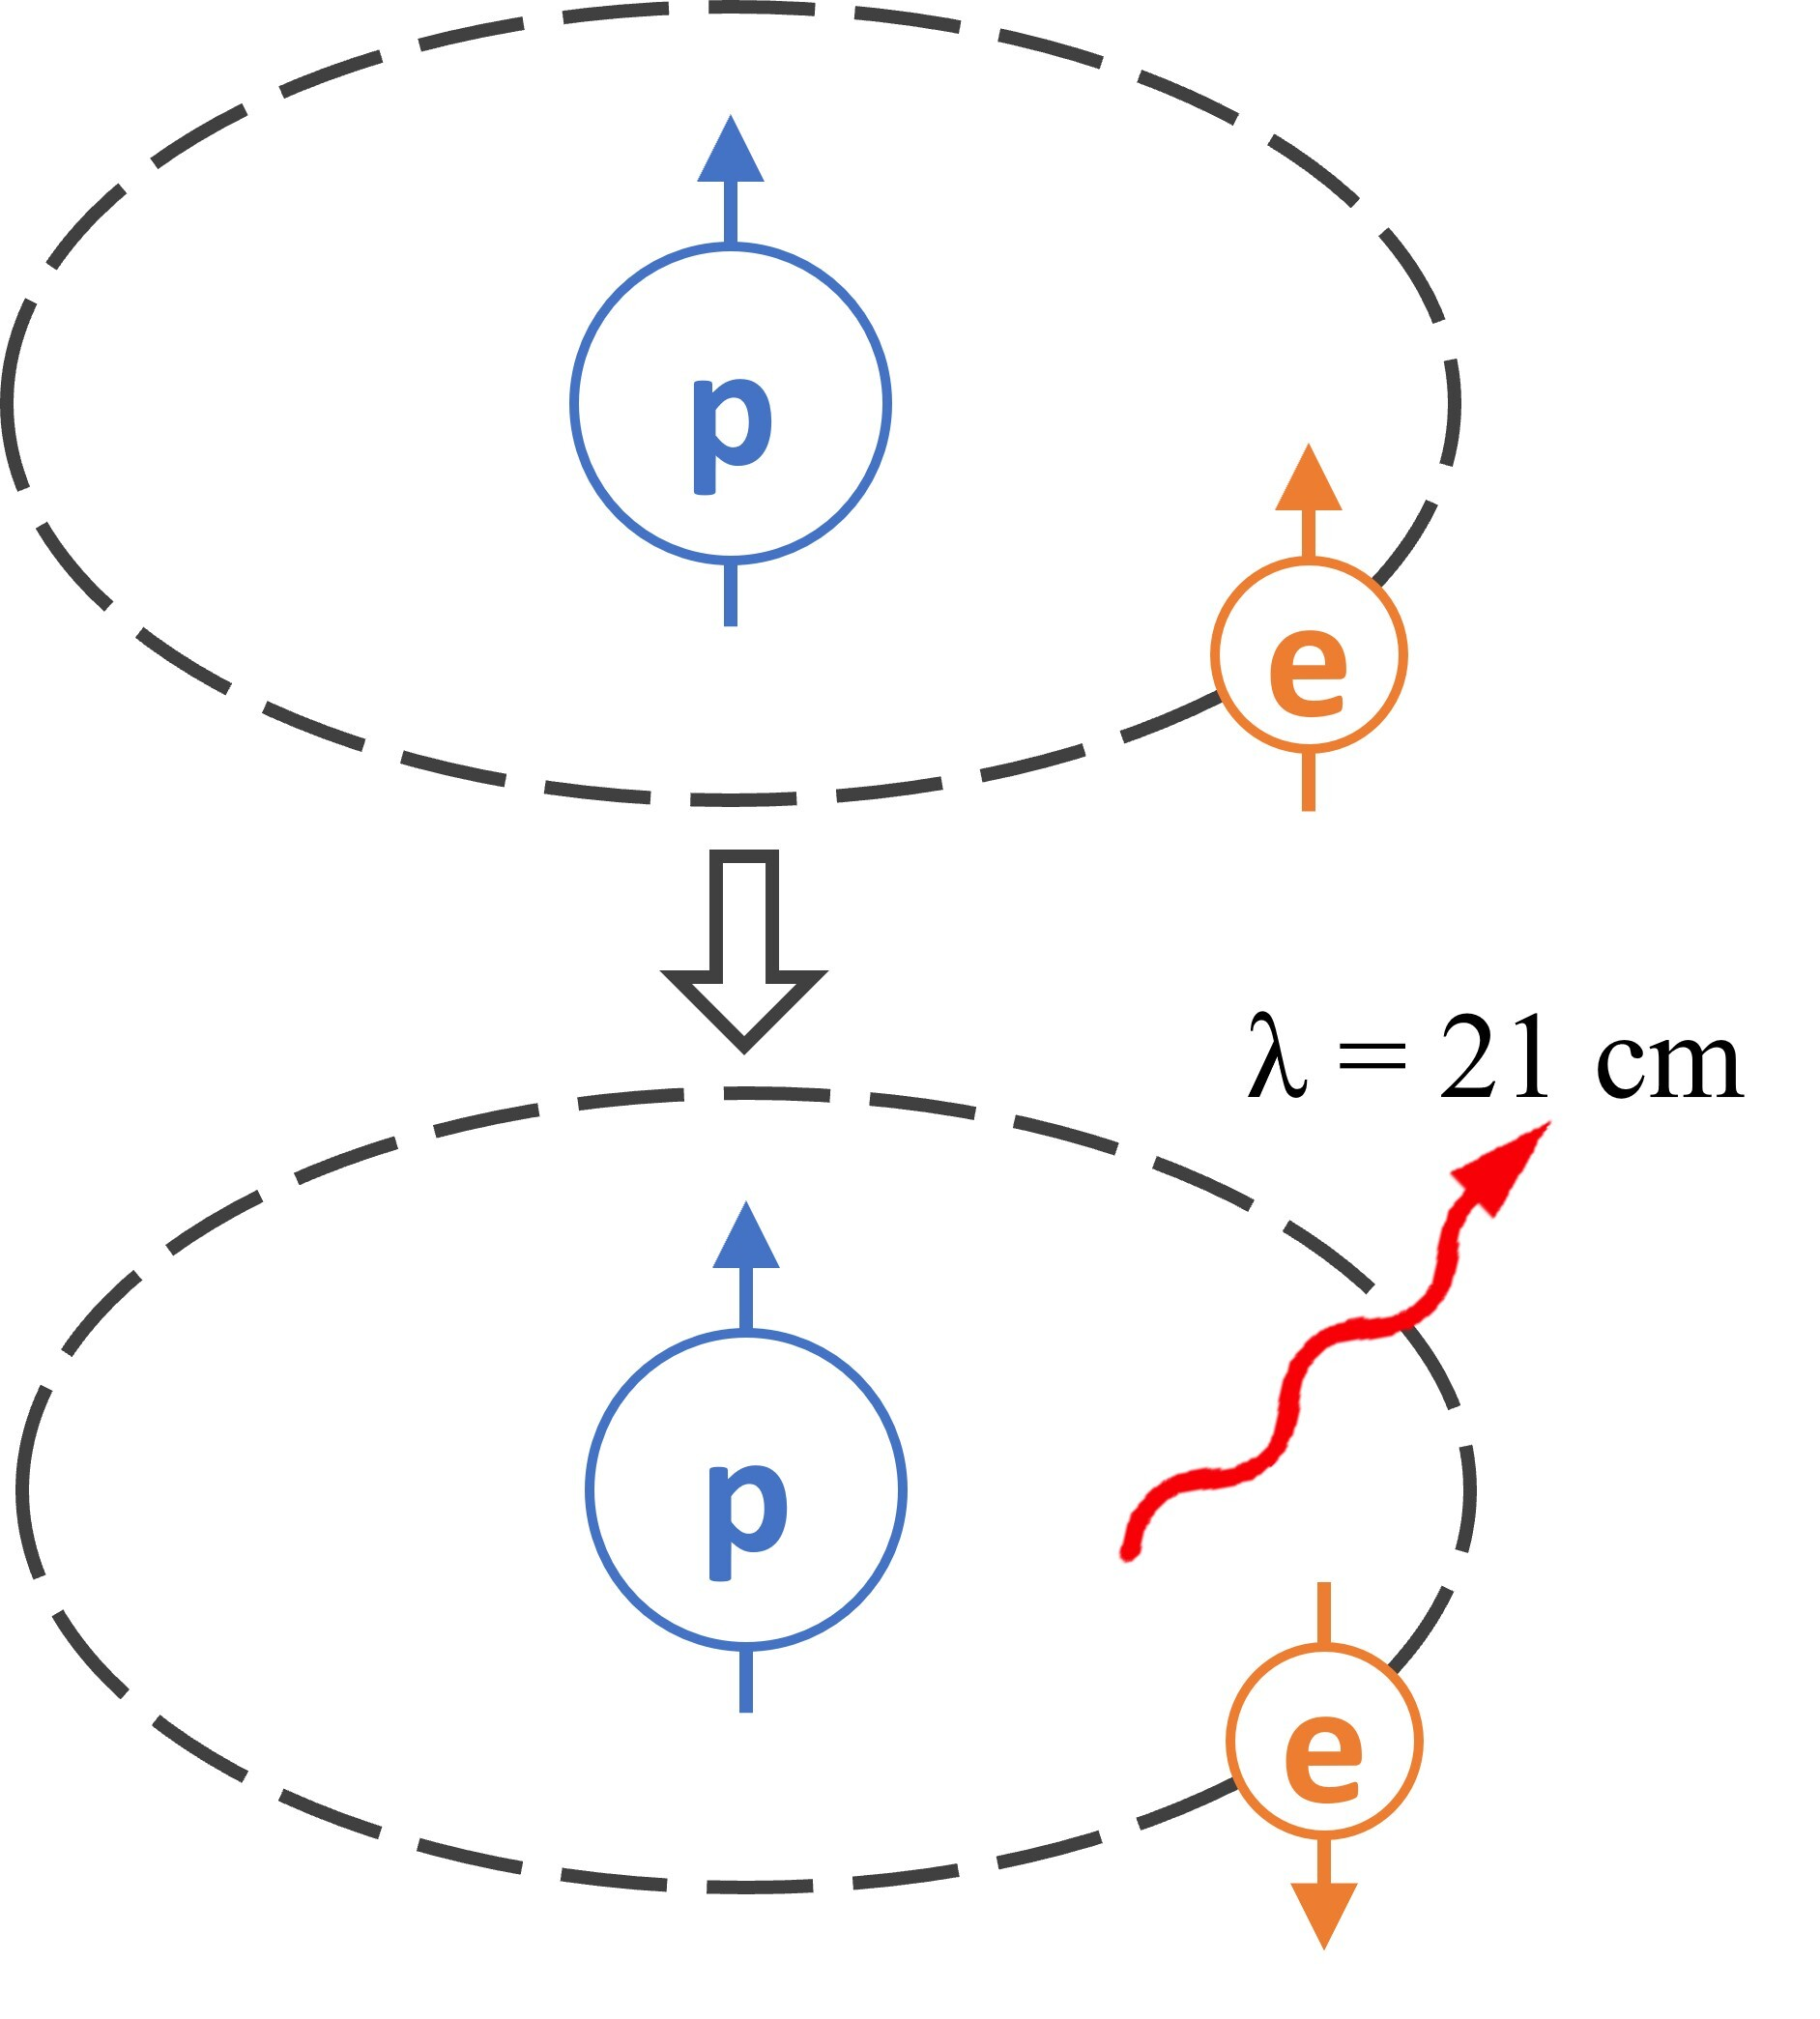
\includegraphics[scale =0.4]{spinflip.jpg}
\caption[Spin-flip Transition of Neutral Hydrogen]{\hl{A basic depiction of the spin-flip transition on the ground energy state of the neutral hydrogen. The upper and lower plots indicate the triplet and singlet states, respectively. The energy difference associated with this transition is $\Delta E = 5.9 \times 10 ^{-6}eV$ }\cite{21century}. Figure from Kit Gerodias \cite{kit_thesis}.}
\label{fig:spinflip}
\end{figure}
\hl{Given that the CMB encompasses photons with the wavelength of $21cm$, hydrogen atoms are able to engage in interactions with the CMB, thereby facilitating the absorption of the $21cm$ photon. This interaction takes place approximately during the dark ages and the EoR. As a consequence of this interaction, the brightness temperature of the $21cm$ line experiences a notable alteration\footnote{This interaction will be discussed in detail in Chapter \ref{chap:global21cm} as the coupling of the spin temperature $T_s$ with the kinetic temperature of the gas $T_k$.}. Using modern radio interferometers equipped with precise observation capabilities, this alteration can be detected effectively. It should be noted that due to the redshift, the 21 cm signal attains frequencies ranging from approximately 30 to 200 $MHz$, rendering it easily accessible to our radio interferometers} \cite{low_frequency}.
These observations are capable of giving us valuable information about the distribution of neutral hydrogen and the evolution of cosmic structure over time\cite{low_frequency}.\par
The global $21cm$ signal is the average over the brightness temperature of the $21cm$ line across the entire sky. It is a measure of the overall state of the intergalactic medium (IGM) and presents itself as an excess absorption or emission in different redshift regions. This radiation is an observational evidence for certain characteristics of the IGM in the early universe (e.g., temperature, density, and reionization state). These properties are determined by the complex interplay between the cosmic radiation field, the formation and evolution of the first stars and galaxies, and the feedback processes that these sources exert on their surroundings\cite{21century}.\par
Besides all the above-mentioned applications, the global $21cm$ signal is a \textbf{strong probe for non-standard physics} during the dark ages. It has the potential to shed light on mysteries surrounding dark matter/dark energy, the existence of cosmic strings, and even certain particle interaction  \cite{dark_nature_21, constrain_dm_21, cosmic_string_brandenberger, ee_interaction_21, neutrino_21} \footnote{These effects will be discussed more in \ref{chap:global21cm,sub:non_standard}.}. This capacity of the global $21cm$ signal is the main motivation of this research.\par
%-----------------------------------------------------------
\section{Research questions and objectives}
The effects of non-standard physics in $21cm$ signal have gained lots of attraction in the recent literature (cite) \todo{Add these citations}. These effects were investigated through the application of analytical and semi-analytical methods. However, the majority of the studies were predominantly analytical in nature, regardless of the observational data (citation).\par \todo{Add these citations}
We aim to fill this research gap by continuing the semi-analytical efforts to simulate the global $21cm$ signal with an aim to prob these non-standard effects. With the recently released data at our disposal \cite{edges}, we use certain fitting algorithms to compare them to theoretically simulated models\cite{ares2014jordan}. 
The first step is to estimate the physical parameters of these curves by only taking the standard physical mechanisms into account.\par
In future studies, we will include a realistic foreground model and upgrade our simulator to include desired non-standard effects. We will again fit the observational data to the upgraded version of the theoretical model to investigate patterns of change in the best-fit physical parameters. The insights from this study will be used to constrain the physical parameters found by the newly proposed models. Moreover, it will empower us to determine whether the upcoming radio interferometers have enough precision to detect our targeted non-standard effects.\par
%-----------------------------------------------------------
\section{Overview of the thesis}
This thesis consists of two major components: the literature review and the research.\par
In the literature review chapters (chapters \ref{chap:global21cm} and \ref{chap:observations}), we first talk about the global $21cm$ signal and its physical principles. We continue by exploring the effects of non-standard physics on the global $21cm$ signal in the recent literature. \par
In chapter \ref{chap:observations}, we will briefly introduce all of the present and future observational projects aiming to detect the global 21cm signal. From all these experiments, we will thoroughly discuss the Experiment to Detect the Global EoR Signature (EDGES) and the Small Array for Research in Astrophysics of the South (SARAS)\footnote{\hl{The selection of these two experiments is justified by their explicit emphasis on observing the global 21cm signal rather than spatial fluctuations, coupled with the availability of their released data.}}.\par
In the research half of this thesis (chapters \ref{chap:method} and \ref{chap:results}), we place a stronger emphasis on computational aspects. 
In chapter \ref{chap:method}, we examine the importance of estimating the parameters of the global $21cm$ signal and how these estimations affect future proposed theoretical models and observations. Furthermore, we briefly describe different methods used to serve this purpose and the advantages of each one.
Subsequently, we will Bring forth the details of the specific method used in this study. 
Chapter \ref{chap:results}, demonstrates the results of applying this computational method to EDGES observational data.\par

Finally, in chapter \ref{chap:discussion}, we interpret the outcome and talk about the implications of these results for cosmology and astrophysics. Also, the limitations and the future prospects of the project are mentioned in this chapter.\par
%###########################################################
\chapter{The Global 21cm Signal}
\label{chap:global21cm}
The $21cm$ cosmology has been a rapidly evolving field of study since its onset in the mid-1900s. Elaboration of this branch of cosmology assists us in forming a better understanding of primordial hydrogen and the physical mechanisms affecting its evolution. Despite the fact that details of the physics behind the $21cm$ line are associated with undeniable uncertainties and the parameter space of the theory is not strictly constrained, the self-consistency and mutual compatibility of the overall structure of the theory guarantee its potential in the future of cosmology. \par
This chapter is specifically dedicated to the investigation of  \textbf{global 21cm signal}. In section \ref{chap:global21cm,sub:physics}, we initiate the discussion by describing the nature of the $21cm$ line and how the related interactions give rise to the global curve. Then we briefly portray the computational efforts in this field by introducing two famous semi-numerical simulations of this radiation.
As we move along to the last section, we pursue our discussion by the latest findings on the signature of non-standard physics on the $21cm$ signal. These effects originate from corresponding theories beyond the standard model of cosmology and particle physics.\par
%-----------------------------------------------------------
\section{Theoretical basis of the 21cm signal}
\label{chap:global21cm,sub:physics}
\subsection{Physical Principles of the 21cm spectral line}
Based on the prior well-accepted knowledge that the $21cm$ signal is a result of interaction between the \gls{cmb} and the matter along its way, we expect the characteristics of the signal to depend on the radiative transfer along the line of sight. As a result, to find the brightness temperature of the $21cm$ line, we start with the basic \gls{rte} for the specific intensity $I_{\nu}$:
\begin{equation}
    \frac{dI_\nu}{ds} = - \alpha_\nu + j_\nu ,
    \label{eq:RT}
\end{equation}
Where $\alpha_\nu$ and $j_\nu$ are absorption and emission coefficients, respectively. It is essential to note that this equation is written under the assumption of zero scattering \cite{21century, low_frequency}. \par
We relate the $I_\nu$ to temperature by the assumption working in Rayleigh-Jeans limit, which gives: $I_\nu = 2k_B T \nu^2 /c^2$. Moreover, the optical depth along the line of sight is defined as: $\int \alpha_\nu \left(s\right) ds$, where $ds$ is a path length. Now, we may rewrite equation \ref{eq:RT} to find the observed brightness temperature $T^{obs}_b$ at a frequency $\nu$ along the line of sight from a background radio source through a cloud of optical depth $\tau_\nu$ and uniform excitation temperature $T_{ex}$ \cite{21century, low_frequency}:
\begin{equation}
    T^{obs}_b = T_{ex} \left(1-e^{-\tau_\nu} \right) + T_R \left (\nu \right) e ^{-\tau_\nu}
\end{equation}
For $21cm$ applications, the excitation temperature is referred to as spin temperature $T_S$. It is defined based on the population (number densities) of hydrogen atoms in the triplet ($n_0$) and singlet state ($n_1$) \footnote{Refer to figure \ref{fig:spinflip} for the definition of hydrogen hyperfine singlet and triplet state.}\cite{21century, low_frequency}.
\begin{gather}
    \frac{n_1}{n_0} = \frac{g_1}{g_0} e ^ {-\frac{T_*}{T_S}}\\
    g_0 =1, g_1 =3\\
     T_* \equiv \frac{E_{10}}{K_B T_S} = \frac {hc}{k\lambda_{21cm}} = 0.068 K
\end{gather}
$g_0$ and $g_1$ are the statistical degeneracy factors, and $T_*$ is a factor with dimensions of temperature defined for convenience. The deviation of the spin temperature from the background temperature is the key to the detectability of this signal\footnote{Although it is possible to choose a radio-loud point source as the background template, however since the order of fluctuations in the \gls{cmb} temperature is insignificant in our study ($\delta T_{CMB} \approx 10 ^{-5}$), the \gls{cmb} is a great candidate as a source of uniform brightness\cite{21century}.}. Thus, in the study of the physics of the $21cm$ signal, we mainly focus on the fluctuations of the spin temperature.\par
With this expression, we calculate the optical depth of a cloud of hydrogen as \cite{21century, low_frequency}:
\begin{gather}
    \tau_\nu=\int \mathrm{d} s\left[1- e^{ \frac {T_*}{ T_S}}\right] \sigma_0 \phi(v) n_0 ,\\
    n_0 =\frac{n_H}{a},\\
    \sigma_0 \equiv \frac{3c^2 A_{10}}{8\pi \nu^2}
\end{gather}
where $\phi_\nu$ accounts for the line profile, normalized so that $\int \phi \left(\nu\right) =1$. $n_H$ is the hydrogen number density, and the $1/4$ factor is the ratio of hydrogen atoms in the hyperfine triplet state. $\sigma_0$ represents the $21cm$ cross-section dependant on the spontaneous decay rate of the spin-flip transition $A_{10} = 2.85 \times 10^{-15} s^{-1}$ \cite{21century, low_frequency}. The very small value of $A_{10}$ implies the rare occurrence of the transition and explains the faintness of the 2cm signal \cite{kit_thesis}. 

Three competing processes influence the spin temperature: 1) interaction of $21cm$ photons with the radio background (mostly \gls{cmb}), 2) collisions with other particles (a mixture of hydrogen atoms, free electrons, and protons with hydrogen atoms as the leading component), and 3) resonant scattering of \gls{lya} photons that cause a spin-flip transition with through the meddling of an intermediate excited state. Therefore, the spin temperature will be expressed using the equilibrium between these mechanisms and their corresponding Einstein coefficients. After algebraic simplifications, we have \cite{low_frequency,21century}:
\begin{equation}
    T^{-1}_S = \frac{T^{-1}_\gamma + x_\alpha T^{-1}_\alpha + x_c T^{-1}_K}{1 + x_\alpha + x_c}.
\end{equation}
Where $T_\gamma$ is the temperature of the surrounding bath of radio photons ($T_\gamma = T_{CMB}$). $T_\alpha$ is the color temperature of the \gls{lya} radiation field (at the \gls{lya} frequency). Normally, it is assumed to have the same value as the gas kinetic temperature $T_K$ as a result of repeated scatterings and their recoils. $x_c$ and $x_\alpha$ are the coupling coefficients due to atomic collisions and scattering of \gls{lya} photons, respectively. The spin temperature becomes strongly coupled to the gas temperature when terms with coupling coefficients become dominant: $x_c + x_\alpha \gtrsim 1$. On the other hand, it relaxes to $T_\gamma$ when the coefficients are relatively small: $x_c + x_\alpha << 1$ \cite{21century, low_frequency}. 
\subsubsection{\gls{wf} Coupling}
As previously mentioned, a hydrogen atom in the early universe is able to interact with \gls{cmb} photons that had frequencies matching the energy gaps of hydrogen atoms, especially in the \gls{lya} band. However, with the onset of star formation, \gls{cmb} will no longer be the only source of photons for the hydrogen atom to interact with. The newly formed compact objects are capable of generating \gls{uv} photons, including \gls{lya}, and reheating the \gls{igm}. These photons are injected into the \gls{lya} frequency band by resonant scattering rather than being redshifted from outside the line. The existence of this second channel increases the coupling ability of the hydrogen-background interaction, further assisting the spin temperature $T_S$ in coupling to $T_K$ \cite{21century, low_frequency}.\par
The process of coupling the spin temperature of neutral hydrogen to the \gls{lya} background is called \textbf{\gls{wf} effect} \cite{barkana2001beginning}\footnote{The \gls{wf} coupling is named after two physicists who independently described the phenomenon in 1952 and 1958: Robert H. Wouthuysen \cite{wouthuysen_original}, and George B. Field \cite{field_original}.}. This process plays a pivotal role in the observability of the global $21cm$ signal during the dark ages by forcing the signal to deviate from the temperature of the \gls{cmb}.\par
The \gls{lya} coupling coefficient, indicating the strength of \gls{wf} effect is expressed as a function of scattering rate $P_\alpha$ \cite{low_frequency}:
\begin{equation}
    x_\alpha = \frac{4P_\alpha}{27 A_{10}} \frac{T_*}{T_\gamma}
    \label{eq:x_a}
\end{equation}

\subsection{Sky-Averaged 21cm Signal}
\label{chap:global21cm,sub:physics,sub:global}
We previously mentioned that the global $21cm$ signal is the average over all the spatial fluctuations of the $21cm$ signal. Generally, we study the behavior of this signal in comparison to a roughly uniform source of radio background. Thus, we define the differential brightness temperature of the global $21cm$ signal as the excess brightness temperature (due to emission or absorption) of the global $21cm$ signal with respect to that of the background, which in our case, is assumed to be \gls{cmb}. Therefore,
\begin{equation}
    \delta T_b = T_{S} - T_{\gamma} = T_S - T_{CMB}.
\end{equation}
Based on the discussions of the last section, this differential brightness temperature is found using the following expression \cite{low_frequency}:
\begin{equation}
    \delta T_b \approx 27 \left(1- \bar{x}_i\right) \left(\frac{\Omega_{b, 0}h^2}{0.023}\right) \left( \frac{0.15}{\Omega_{m, 0}h^2} \frac{1+z}{10}\right)^{1/2}\left(1-\frac{T_\gamma}{T_S}\right)
    \label{eq:global_curve}
\end{equation}
Where $x_i$ is the ionization fraction, and $h$ is the dimensionless Hubble constant. $\Omega_{b, 0}$ and $\Omega_{m, 0}$ are the ratio of the current energy density of baryonic and total matter with respect to the critical energy density of the universe.\par
To further investigate the fluctuations of the global $21cm$ through the thermal history of the universe and the physical mechanisms behind the troughs, we split the early universe era into different redshift regions\footnote{It is crucial to mention that there is still considerable uncertainty in the exact values of the redshift bounds and the sequence of events due to our highly limited knowledge on the characteristics and effects of early sources. This uncertainty is such significant that there might even be an overlap between these discussed regions \cite{21century}.}:\par
\begin{itemize}
\item $200 \lesssim z \lesssim 1100$: The universe is filled with high-density gas and the residual free electrons from the recombination. Compton scattering maintains the thermal coupling of gas to \gls{cmb} temperature through the electrons ($T_K = T_\gamma$). Due to the high density, the collisional coupling is dominant, forcing the spin temperature to the kinetic temperature of the gas ($T_S = T_K$). 
Therefore, the differential brightness temperature of the $21cm$ signal is zero during this redshift regime ($T_S = T_\gamma$)\cite{21century}.\par

\item $40 \lesssim z \lesssim 200$ (Dark Ages): The universe becomes cool enough for subatomic particles to combine and form neutral hydrogen. As a natural result, baryonic matter experiences thermal decoupling from the \gls{cmb}, making it possible for the non-relativistic gas to cool adiabatically with the expansion of the universe \cite{21century}. The temperature of the gas and \gls{cmb} drops as $T\propto a^{-2}$ and $T\propto a^{-1}$ respectively\footnote{"\emph{a}" is the expansion scale factor.}. This rate discrepancy leaves the gas cooler than radiation while effectively stopping heat exchange between these two components. Therefore, the gas spin temperate decouples from that of \gls{cmb}. Since collisional coupling is still significantly strong, the spin temperature remains in coupled to the gas kinetic temperature ($T_S = T_K$). Consequently, the $21cm$ differential brightness temperature becomes negative (absorption) in this redshift region \cite{map_universe, 21century}.\par

\item $z_* \lesssim z \lesssim 40$: As the density keeps dropping through the expansion, the influence of collisional couplings becomes less significant, causing the spin temperature to again couple with the \gls{cmb} temperature ($T_S \rightarrow T_\gamma$). Thus, the $21cm$ differential brightness signal goes back to zero again\cite{map_universe}. The first blue regions in the upper panel of figure \ref{fig:global_signal_pritchard_loeb} and the corresponding absorption trough in the lower panel depict the above-mentioned process \cite{map_universe, 21century}.\par

\item $z_\alpha \lesssim z \lesssim z_*$: The second trough in figure \ref{fig:global_signal_pritchard_loeb} emerged through the formation of the first structures. As large halos begin to collapse to form first stars and galaxies, they generate both x-ray and \gls{lya} emissions. Two mechanisms create the \gls{lya} photons: 1) Continuous redshifting of background radiation to the \gls{lya} wavelength and 2) Ionization and deexcitation of \gls{igm} gas. Since the emissivity required for the \gls{lya} coupling is significantly less than that for heating $T_k$ above $T_\gamma$, the spin temperature tends to couple to cold gas ($T_S \rightarrow T_K$) through the \gls{wf} effect. Therefore, we will again observe the global $21cm$ signal in absorption \cite{map_universe, 21century}.\par

\item $z_r \lesssim z \lesssim z_\alpha$ (Reionization): Eventually, the gas is reheated by ionizing x-ray photons from early sources \cite{21century}, and the $21cm$ differential brightness temperature goes back to zero (second absorption trough in the lower panel of figure \ref{fig:global_signal_pritchard_loeb}). The influence of this reheating mechanism is such strong that we even expect to observe $21cm$ emission in this redshift range (red region in the upper panel of figure \ref{fig:global_signal_pritchard_loeb}). From this point on in the thermal history of the universe, we do not expect to see any more $21cm$ radiation from IGM since the majority of the gas will be ionized by emergent stars, galaxies, and accreting black holes. Therefore, the $21cm$ differential brightness temperature goes to zero (the black region in the upper panel of figure \ref{fig:global_signal_pritchard_loeb}). However, in the regions with higher recombination rates inside galaxies and dark matter halos, the neutral hydrogen is shielded and preserved. Consequently, the 21cm signature originating from inside the galaxies will continue to be emitted\cite{map_universe, 21century}.\par
\end{itemize}
\begin{figure}[h!]

\centering
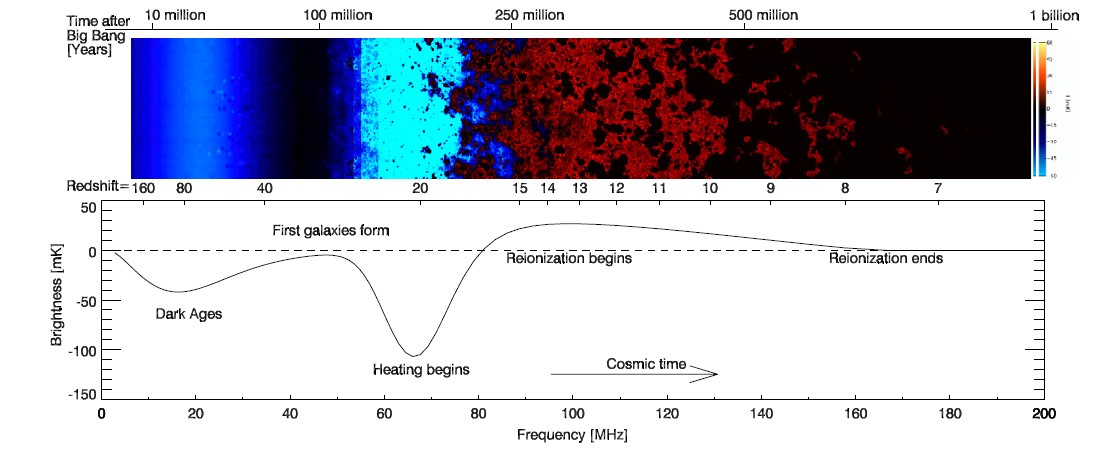
\includegraphics[scale =0.8]{global_signal_pritchard_loeb.jpg}
\caption[Time evolution of the fluctuations in the $21cm$ differential brightness temperature]{Time evolution of the fluctuations in the $21cm$ differential brightness temperature (solid line). The top panel is a color plot demonstrating fluctuations arising from variations in density. The coloration clearly depicts the two absorption phases of $21cm$ brightness temperature (coupling of $T_S$ to $T_K$, blue regions), emission phase (red regions), and the interval where it disappears completely (coupling of $T_S$ to $T_\gamma$, black region). The lower panel represents the evolution of sky-average (global) $21cm$ signal from the dark ages to the reionization. The frequency range of the absorption and emission regions exactly matches the corresponding regions in the upper panel. The precise details of the shape of this signal are still unidentified due to our lack of knowledge on the nature of early sources\cite{liu2013global}. Figure from Pritchard and Loeb, 2011 \cite{21century}.}
\label{fig:global_signal_pritchard_loeb}
\end{figure}
%-----------------------------------------------------------
\section{Simulating the global 21cm signal}
With the current advancements in radio telescope instrumentation, we have entered a data-driven era in $21cm$ cosmology, empowering us to constrain the properties of astrophysical sources responsible for generating this signal. Nevertheless, extracting astrophysical insights from the collected data is a complex task that necessitates the fast and efficient generation of theoretical templates spanning over the parameter space \cite{emulate_21cm}. \par
To reach this purpose, fully hydrodynamic simulations of the 3-dimensional evolution of the $21cm$ signal have been adapted\cite{21cmfast_c}. However, these simulations are computationally expensive, and this restriction will considerably decrease our ability to search the parameters space \cite{ares2014jordan}. 
Semi-analytical methods are the proposed state-of-the-art solutions employing a middle-ground approach between these simulations and fully analytical studies. The results of these semi-analytical calculations are in remarkable agreement with corresponding hydrodynamic simulations while consuming a significantly lower amount of run-time. \par
In this section, we introduce two powerful tools capable of simulating the theoretical $21cm$ curves over a wide range of astrophysical and cosmological parameters. The first one is \gls{21cmfast}, which is a popular tool to simulate the spatial fluctuations of $21cm$ signal. It is also capable of generating the global curve by averaging over all the signals in different directions. The other one is the \gls{ares}, which calculates the global curve directly, using a novel approach to solving the cosmological \gls{rte} \cite{ares2014jordan}. Although \gls{21cmfast} is perfectly capable of doing the same tasks as \gls{ares}, we prioritize the utilization of \gls{ares} in our analysis. The rationale is based on the fact that employing the \gls{21cmfast} is considered to be excessive for generating the global $21cm$ curve.\par

\subsection{21 Centimeter Fast Approximate Signal Toolbox (21cmFAST)}
\gls{21cmfast} is a Python-integrated C package designed to produce 3D cosmological realizations of physical fields playing a role in the early universe. It is based on a semi-numerical approach combining the excursion set formalism with perturbation theory. \gls{21cmfast} is capable of simulating the 3D realizations of density, peculiar velocity, halo, ionization, spin temperature fields, $21cm$, and ionizing flux fields\footnote{Documentation: \hyperlink{https://21cmfast.readthedocs.io/en/latest/}{https://21cmfast.readthedocs.io/en/latest/}}\footnote{GitHub Repository: \hyperlink{https://github.com/21cmfast/21cmFAST}{https://github.com/21cmfast/21cmFAST}} \cite{21cmfast_c, 21cmfast_python}.\par
As mentioned above, the original simulation was developed as a C script. Later, in 2020, the equivalent Python package was introduced as the third version of \gls{21cmfast}. The core C code is a high-performance script aiming to identify regions of ionized hydrogen in a complex cosmological density field based on excursion set formalism. The evolution of the field is analyzed using first- or second-order Lagrangian perturbation theory. Taking this approach will result in revealing the history of thermal and ionization states of IGM, alongside X-ray, and \gls{uv} radiation fields, derived from galaxy models \cite{21cmfast_c}. \par
An example of a mean temperature curve generated using \gls{21cmfast} is shown in \ref{fig:21cmfast_curve}.
\begin{figure}[h!]
    \centering
    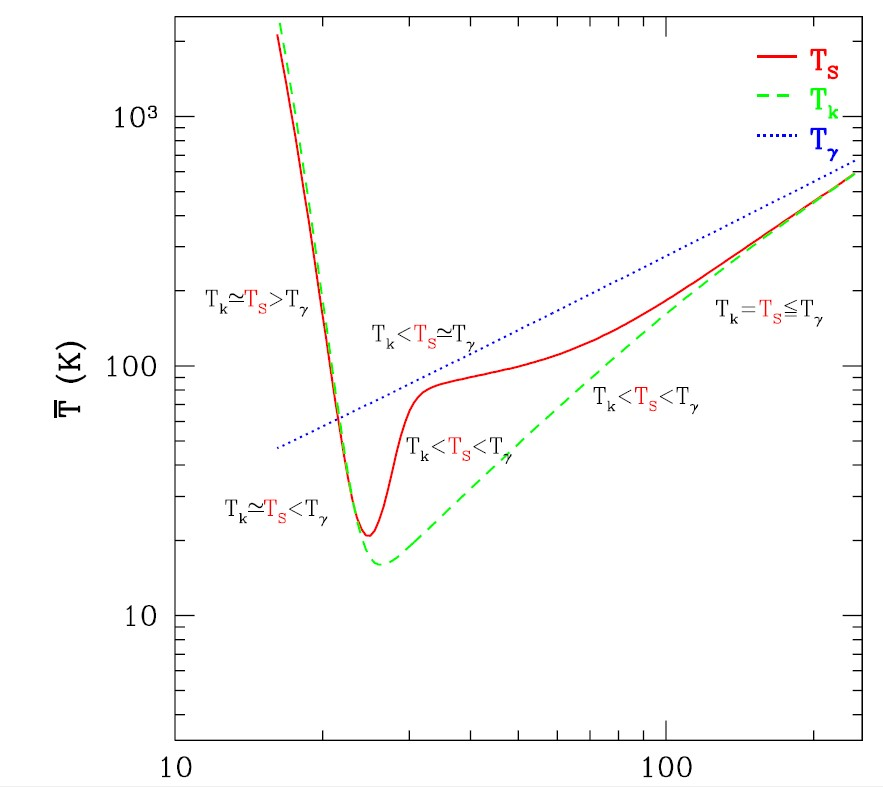
\includegraphics[scale = 0.6]{21cm_curve.jpg}
    \caption[Evolution of the mean temperature generated using \gls{21cmfast}]{Evolution of the mean temperature generated using \gls{21cmfast}. Solid, dotted, and dashed curves represent the spin temperature, CMB temperature ($T_\gamma$ or equivalently $T_CMB$), and the kinetic temperature of the gas, respectively. Figure from \cite{21cmfast_python}}
    \label{fig:21cmfast_curve}
\end{figure}
\subsection{The Accelerated Reionization Era Simulations (ARES)}
The Accelerated Reionization Era Simulations, or in the short form \emph{\gls{ares}}, is a Python package for generating global $21cm$ curves \footnote{Documentation: \hyperlink{https://ares.readthedocs.io/en/latest/}{https://ares.readthedocs.io/en/latest/}} \footnote{GitHub Repository: \hyperlink{https://github.com/mirochaj/ares}{https://github.com/mirochaj/ares}}\cite{ares2014jordan}. Alongside this applications, it can be used for stand-alone non-equilibrium chemistry solver, global radiation background calculator,  galaxy semi-analytic modeling \cite{jordan_galaxy_1, jordan_galaxy_2, jordan_galaxy_3}, PopIII star modeling \cite{jordan_star}, 1D radiative transfer, and \gls{sed} optimization \cite{jordan_SED}.\par
\gls{ares} draws the globally-averaged $21cm$ curve through the numerical calculation of differential brightness temperature $\delta T_b$ (equation \ref{eq:global_curve}). This approach necessitates the evolution of the spin temperature $T_S$, which itself is dependent on coupling coefficients $x_\alpha$ and $x_c$. The collisional coupling coefficient $x_c$ is found using the tabulated values in \cite{ares_collision_coeff}, and the \gls{lya} coupling coefficient is calculated from equation \ref{eq:x_a}. By ignoring detailed line profile effects, this expression can be written in the following form as a function of angle-averaged $Ly\alpha$ back-ground intensity $\widehat{J}_\alpha$, which determines the strength of Wouthuysen-Field coupling \cite{ares2014jordan, ares_lya_coeff_1, ares_lya_coeff_2, ares_lya_coeff_3}:  
\begin{equation}
    x_\alpha = 1.81 \times 10^{11} \frac{\widehat{J}_\alpha}{1+z}
    \label{eq:x_a}
\end{equation}
Where $\widehat{J}_\alpha$  is a specification of the general definition of angle-averaged back-ground intensity as a function of co-moving volume density emissivity \cite{ares2014jordan}:
\begin{equation}
    \widehat{J}_\nu (z)=\frac{c}{4 \pi}(1+z)^2 \int_z^{z_{\mathrm{f}}} \frac{\hat{\epsilon}_{\nu^{\prime}}\left(z^{\prime}\right)}{H\left(z^{\prime}\right)} \mathrm{e}^{-\bar{\tau}_\nu} \mathrm{~d} z^{\prime}
    \footnote{In this expression the $\widehat{J}_v(z)$ and $\hat{\epsilon}_{\nu^{\prime}}$  are in units of photon number density:
    $\left[\hat{J}_v\right]=\mathrm{s}^{-1} \mathrm{~cm}^{-2} \mathrm{~Hz}^{-1} \mathrm{sr}^{-1}$,
    $\left[\hat{\epsilon}_v\right]=\mathrm{s}^{-1} \mathrm{~Hz}^{-1} \mathrm{cMpc}^{-3}$.} 
\end{equation}  
Numerical evaluation of this expression is generally computationally heavy, mostly due to the optical depth ($\tau_\nu$) term. A clever solution is to tabulate the optical depth values on an arbitrary number of redshift points. However, the accuracy of this method is dependent on the number of chosen redshift points in the look-up table, and undersampling might result in large deviations in background radiation intensity.\par
In summary, \gls{ares} simulates the behavior of \ref{eq:global_curve} as a function redshift and portray the global $21cm$ signal. A typical \gls{ares}-generated curve is presented in \ref{fig:ares_Curve}. \par
\begin{figure}[h!]
    \centering
    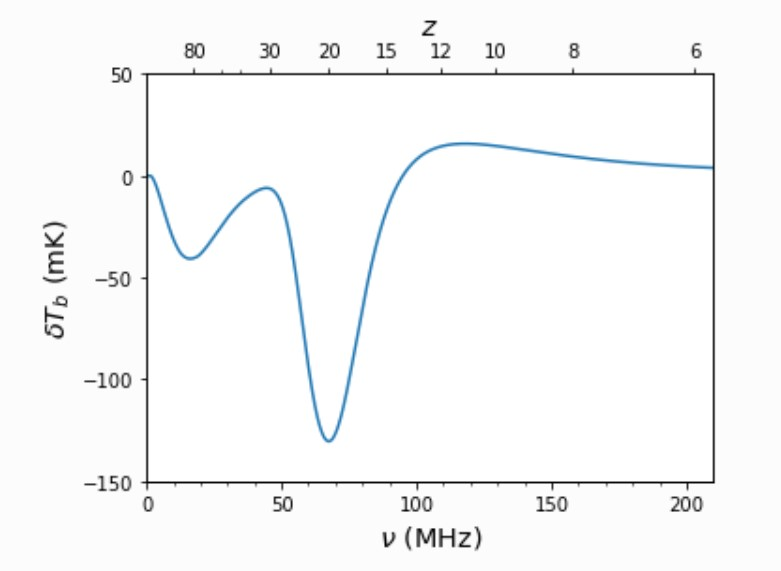
\includegraphics[scale =0.8]{ares_curve.jpg}
    \caption[Typical global $21cm$ curve generated using \gls{ares}]{An example of a global $21cm$ signal generated using \gls{ares}, illustrating the evolution of the brightness temperature of $21cm$ line against the background radio sources as a function of frequency/redshift. The fluctuations discussed in section \ref{chap:global21cm,sub:physics,sub:global} are perfectly demonstrated in the simulated signal. Note the similarities to corresponding regions in figure \ref{fig:global_signal_pritchard_loeb}. Figure from Jordan Mirocha in the \hyperlink{https://ares.readthedocs.io/en/latest/examples/example_gs_standard.html}{ARES documentation}}
    \label{fig:ares_Curve}
\end{figure}
%------------------------------------------------------------
\section{Effects of non-standard physics on the global 21cm signal}
\label{chap:global21cm,sub:non_standard}
%add the effects of primordial magnetic fields
The physics of the $21cm$ signal indicates that if the \gls{igm} ionization state is close to neutral and the coupling is saturated, the brightness temperature of this line is strongly dependent on the temperature fluctuations of the \gls{igm}. Therefore, any physical process involving heat exchange with the \gls{igm} is expected to print their signature on the $21cm$ global signal \cite{21century}. Many proposed models of physics beyond the standard model of cosmology and particle physics predict this exotic heating of the 
\gls{igm} \cite{21century}, Therefore, we dedicate this section to the investigation of these effects. The exact calculation of these fluctuations on the $21cm$ signal will determine the ability of upcoming observational data to detect these effects.\par
Among these beyond standard models, different dark matter candidates play a pivotal role. For example, it is expected that decaying or annihilating dark matter and evaporation of primordial black holes can inject energy into the \gls{igm} and lead to a stronger brightness temperature of 21cm signal through the \gls{eor}. Therefore, we might be able to constrain these theories by observing their features on the global $21cm$ signal \cite{primordial_bh, new_physics_thesis, primordial_bh_binary, 21limit_dm_bh, bound_dm} or even rule out some of these candidates \cite{rule_out}.\par
Another significant effect comes from the interactions associated with cosmic strings. The non-linear gravitational influence of cosmic string wakes or the decay of cosmic string cups is considered a source of exotic heating for the \gls{igm} \cite{cosmic_string_oscar, string_loop_robert}. \par
Moreover, rapidly growing radio-luminous black holes of intermediate mass emit radio signals on their way to becoming supermassive black holes. Thus, they are a type of astrophysical radio source with the ability to enhance the amplitude of the global $21cm$ signal \cite{bh_cosmioc_dawn} \footnote{The author of \cite{bh_cosmioc_dawn} claims that the effect of rapidly growing radio-luminous black holes is a reasonable explanation for the signal reported by \gls{edges}}. \par
In the remainder of this section, we will focus on two of these distinctive non-standard effects, which attracted the attention of the majority of recent literature related to this ares of research.\par

\subsection{Dark Matter (DM)}
%I can add some newer papers to this section, from the new directory in my Zotero library
The majority of the proposed \gls{dm} candidates encompass physical mechanisms capable of affecting the baryon temperature of the ionization state during the cosmic dawn. These features can be employed to reveal the interactions of \gls{dm} with the visible sector. Formerly, \gls{cmb} power spectra were used to investigate these signatures. However, the $21cm$ background can probe energy injection rates approximately above $10^{-24}eV cm^{-3} sec^{-1}$, which is a much higher sensitivity compared to \gls{cmb} power spectra.\par
Decaying or annihilating \gls{dm} produces a secondary source for high-energy particles which, in fact, can heat and ionize the \gls{igm}, contribute to the \gls{lya} background, and leave an imprint on $21cm$ signal. \par
Among these various candidates, decaying or annihilating \gls{dm} may eject energy into the \gls{igm} through the interaction of \gls{dm} particles with known standard model particles. The primordial black hole can also thermally interact with the \gls{igm} in the process of Hawking evaporation and the associated radiations. These effects may lead to a stronger brightness temperature of $21cm$ signal through EoR.  Therefore, we might be able to constrain the characteristics of these theories by their absorption feature in the global 21cm signal (e.g., the lifetime of sterile neutrinos \cite{sterile_neutrino}) \cite{primordial_bh, new_physics_thesis, primordial_bh_binary, 21limit_dm_bh, bound_dm} or even rule out some of the possible candidates (e.g., $3 Kev$ warm \gls{dm} \cite{rule_out}). Some studies even go further and suggest that the use of the $21cm$ gradient alongside its brightness temperature is more efficacious for this purpose \cite{DM_anihilation_furlantto, constrain_dm_21, DM_anihilation_1, DM_ionize, dark_cosmology_21, snowmass_dm}.\par

It must be noted that the presence of additional heating during very high redshifts has the potential to elevate $T_k$ along a higher adiabatic path during the era of collisional decoupling. As a result, this diminishes the depth of the absorption trough around $20 \lesssim z \lesssim 20$. Additionally, if \gls{dm} annihilations contribute to \gls{lya} pumping and heating, the observed signal would exhibit a smoother progression throughout the absorption epoch. A roughly similar process takes place in other extreme astrophysical models with enhanced production of hard X-rays. This degeneracy is an issue in distinguishing the signature of annihilating \gls{dm} in the global $21cm$ signal. However, the spatial distribution of these two heating sources is different, making it possible to differentiate them \cite{dark_nature_21}. \par

Moreover, it has been proved that particle \gls{dm} scenarios featuring a suppressed power spectrum of an astrophysical parameter delay the process of star formation. Since the generation of global $21cm$ signal is dependent on the \gls{uv} radiation of first stars, the corresponding absorption through will occur later than expected. This consequence is stronger in non-cold \gls{dm} models, and their absorption signal models are consistently shifted towards smaller redshifts compared to \gls{cdm}. Therefore, The amount by which the signal is delayed can be used to test non-cold \gls{dm} models  \cite{noncold_dm_21, first_star_impact, dm_timing}.\par 

\begin{figure}[h!]
    \centering
    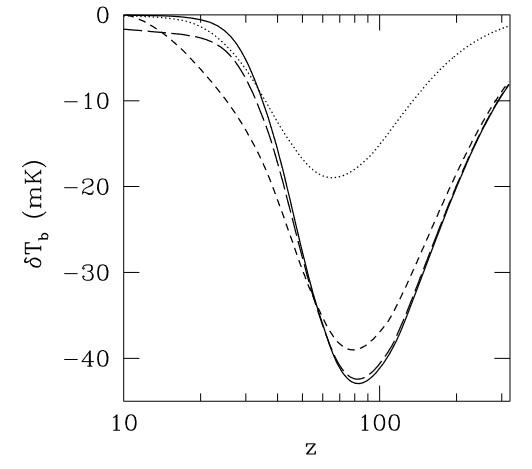
\includegraphics{21cm_dm.jpg}
    \caption[Effect of different \gls{dm} models on the global $21cm$ differential brightness temperature curve]{Effect of different \gls{dm} models on the global $21cm$ differential brightness temperature curve. The solid line shows $\delta T_b$ without decaying/annihilating \gls{dm}, while the long dashed, short dashed, and dotted lines refer to $\delta T_b$ with $25keV$ sterile neutrino decaying \gls{wdm}, $10 MeV$ decaying \gls{ldm}) and $10MeV$ annihilating \gls{ldm}, respectively. Figure from \cite{constrain_dm_21}.}
    \label{fig:enter-label}
\end{figure}



\subsection{Cosmic Strings}
 Cosmic strings are hypothetical one-dimensional topological defects in space-time that are predicted as the solution of the field equation in many theories beyond the standard model of particle physics. They are thought to be formed during phase transitions in the early universe \cite{bryce_thesis, constrain_superconduct}.
 It is expected that cosmic strings leave a distinguished signature on the $21cm$ signal in the form of wedge-shaped regions of extra emission or absorption, depending on the value of string tension. The capability of $21cm$ experiments in accessing higher redshift regions (compared to optical large-scale structure surveys) makes them a perfect candidate to search for the effects of cosmic strings $G\mu$  \cite{cosmic_string_brandenberger, structure_cosmic_string}.\par
Moving strings make wake regions in space-time. The non-linear gravitational effects of this region enhance baryon density \footnote{Cosmic strings are also expected to speed up the process of reionization due to their early generation of non-linear overdensities\cite{corre_21cm_cmb}.}. Higher density increases the collisional coupling, and the spin temperature $T_S$ tends to decrease in these regions, causing a stronger coupling to gas kinetic temperature $T_K$ compared to the surrounding \gls{igm}. In order words, the \gls{wf} coupling is stronger in the presence of cosmic strings. With the assumption that x-ray heating is not significant in the \gls{igm}, the brightness temperature of the $21cm$ signal will be at least two times more negative when the effects of cosmic strings are included. For string tensions $G\mu \gtrsim 3\times 10^ 8$, the enhancement is expected to be larger than noise \cite{WF_effect_oscar}. In lower redshifts, the signature of the cosmic string wakes effect is expected to be more evident since string wake width increases as a function of time, resulting in higher gas temperature and a higher 21cm signal \cite{cosmic_string_brandenberger}.
By calculating the contribution of cosmic string network rather than a single string wake, it was found that the amplitude of the global $21cm$ signal will be enhanced between 10\% to a factor of 2 for string tension in the range of $10^{-8}\lesssim G\mu\lesssim10^{-7}$  \cite{cosmic_string_oscar}.
The assumption of shock-heated cosmic string scenario yields an even stronger \gls{wf} coupling (and hence a stronger $21cm$ brightness temperature with a larger amplitude); however, the effect from a diffuse wake is extended over a wider redshift interval \cite{oscar_robert_shock, WF_effect_oscar}. \par

Cosmic string loops are also expected to imprint a roughly elliptical region in redshift with an extra $21cm$ emission \cite{string_loop_robert}.
It is also viable to study the relevant features in the power spectrum of the $21cm$ signal. Calculations prove that the cosmic string $21cm$ power spectrum turns over at smaller scales compared to the inflationary adiabatic $21cm$ power spectrum \cite{super_string}. Overall, since non-Gaussianities in the distribution of strings (that result in a clearer signature) are only visible in position space, they appear to be a superior choice for such studies \cite{cosmic_string_brandenberger}.\par

Another idea is to study this effect in the cross-correlation of $21cm$ radiation, and \gls{cmb} since their existence will simultaneously fluctuate both signals. The cross-correlation observation of these signatures is more reliable compared to individual signals and can be considered evidence of new physics. Unfortunately, the \gls{cmb}-$21cm$ cross-correlation signal might be overwhelmed by sky temperature noise for observationally allowed cosmic string wakes \cite{corre_21cm_cmb}.

Some studies have computed the contribution of electromagnetic radiation of annihilating super-conducting cosmic strings \footnote{In some models of strings, strings carry conserved electromagnetic currents. Thus, they are superconducting \cite{constrain_superconduct}.}  to the radio background and derived constraints on the parameter space of superconducting cosmic strings \cite{constrain_superconduct, constrain_spectral_bryce, massive_BH}. The assumption of the existence of super-conducting cosmic strings will result in two absorption troughs in the 21cm global signal in $z=20$ and $z\approx 80$. The former exactly corresponds to the trough reported by \gls{edges} for string tension of $G\mu = 10 ^{-10}$. However, the slope on the low redshift end tends to be smoother than that of \gls{edges} data. Astonishingly, the corresponding string tension is the same order of magnitude as the upper bound reported by pulsar riming array measurements \cite{cosmic_string_jordan_robert, pulsar_timing}. The results of this study are shown in figure \ref{fig:21cm_cosmic_string}.\par
Another possibility is to investigate the effect of decay of cosmic string cusps (ordinary string loops \cite{massive_BH}) on the global $21cm$ signal. As calculated by \cite{robert_cusps}, the depth of the absorption through will only be modified by one part in $10^4$ considering this scenario, which is too weak to constrain the parameter space of the proposed theory.\par
\begin{comment}
    This analysis was conducted assuming the fact that the amplitude of the global $21cm$ signal is lower than that obtained by the EDGES collaboration. Their analysis derives out an additional region of parameter space, but the constraints are generally weaker than the ones which follow from pulsar timing array measurements \cite{constrain_superconduct}.
\end{comment}
\begin{figure}[h!]
    \centering
    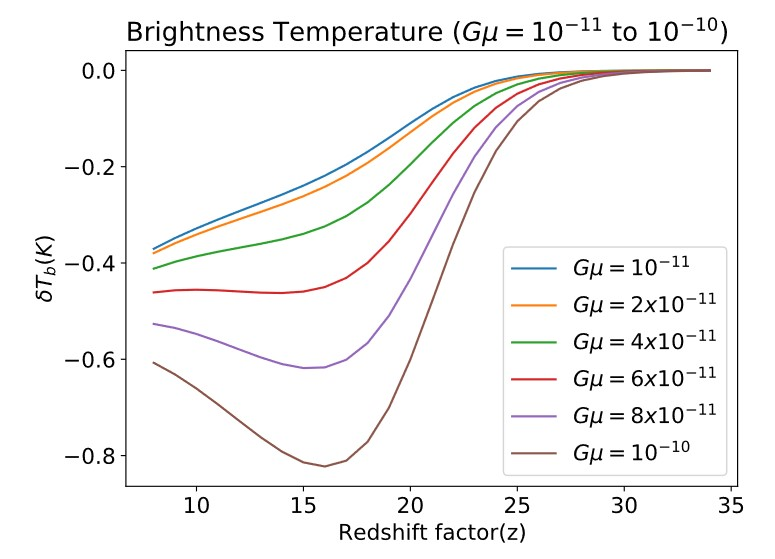
\includegraphics[scale = 0.8]{21cm_cosmic_string.jpg}
    \caption[The global $21cm$ for different values of cosmic string tension]{The differential brightness temperature of $21cm$ signal as a function of redshift for 6 different values of cosmic string tension. The electromagnetic radiation emitted from the decay of superconducting cosmic strings modifies the radio background based on the value of string tension. For the critical tension value of $G\mu = 10 ^{-10}$, the through approaches that of \gls{edges} data. Figure from \cite{cosmic_string_jordan_robert}.}
    \label{fig:21cm_cosmic_string}
\end{figure}

%##############################################################
\chapter{Observations of the Global 21cm Signal}
\label{chap:observations}
List of experiments (reminder: rephrasing and citing each of them,  things that I need for each experiment: dipole antenna, location, time frame of results, frequency range), only mention the global 21cm ones not all 21cm:\par
why is it hard: Unavoidable (beam-averaged)
foregrounds which are > ~10%
times larger than the signal.
• Beam chromaticity mixes spatial
and spectral structure of the
foregrounds with that of the
instrument.
• Also: Ionospheric effects (see
Datta et al. 2016), RFI, radio Solar
emissions.\par
 While most experiments in this field focus on spatial fluctuations of the 21cm signal to study the large-scale structure of the universe, there are a few experiments specifically designed to detect the global $21cm$ signal:
\begin{enumerate}
\item EDGES (Experiment to Detect the Global EoR Signature): This was the first experiment to report a detection of the global 21cm signal in 2018, by measuring the absorption of radio waves from distant sources by neutral hydrogen in the intergalactic medium \cite{edges}.

\item SARAS (Small Array for Research in Astrophysics of the South): This is a radio telescope located in India that has been used to study the global 21cm signal since 2015.

\item PRIZM \cite{prizm_2017} (Probing Radio Intensity at high-Z from Marion): is an experiment that has been designed to study cosmic dawn in the universe using 50-150 MHz observations of globally averaged 21-cm emission. The experiment consists of two modified four-square antennas, operating at center frequencies of 70 and 100 MHz, and a dual-polarization spectrometer back end. PRIZM deployed in April 2017 to Marion Island, an exceptionally isolated and radio-quiet location in the sub-Antarctic, and science observations are currently in progress.
initially called SCI-HI (Small Radio Telescope for Cosmic Hydrogen Intensity Mapping)
\item REACH (Radio Experiment for the Analysis of Cosmic Hydrogen)

\item SKA \cite{SKA_global_21}

\item BIGHORNS (Broadband Instrument for Global HydrOgen ReioNisation Signal): This is a radio interferometer located in Australia that was designed to detect the global 21cm signal during the epoch of reionization.

\end{enumerate}
%--------------------------------------------------------------
\section{Experiment to Detect the Global EoR Signature (EDGES)}
put a picture of the antenna
\subsection{error bars and foreground removal}
\subsection{theoretical model and associated parameters}
%---------------------------------------------------------------
\section{Small Array for Research in Astrophysics of the South (SARAS)}
put a picture of the antenna
%#################################################################
\chapter{Parameter Estimation Methods}
\label{chap:method}
talk about different methods used to serve this purpose and advantages of each one\par
Now that we have talked about the theoretical global 21cm signal and the attempts to observe it, we shall proceed by talking about the parameter estimation of this signal. Various computational algorithms, including machine learning and neural networks, have been used to accomplish this task (cite) \todo{Add the citation}. While neural networks have been shown to be effective, certain drawbacks \todo{mention which draw backs} put sampling algorithms like MCMC on an advantaged position for global 21cm applications.\par
Sampling algorithms like MCMC allow us to map out the full likelihood surface which in our case, is achievable. However, neural nets are usually preserved for problems in which mapping the whole likelihood surface  becomes too complicated.
In this chapter, we describe the main fitting algorithm used in our study, which combines Levenberg-Marquardt and MCMC. We explain the reason behind utilzing both of these algorithms for this particular fitting challenge and provide a detailed explanation of the procedure to combine them. We also discuss two different tests used to measure the quality of the proposed fit.\par
In chapter \ref{chap:results}, we present the results of applying this fitting method to the observed global 21cm curve\footnote{released by the EDGES group} and its corresponding theoretical model\footnote{generated using ARES}.
%------------------------------------------------------------------
\section{Levenberg-Marquardt (LM)}
\label{chap:method,sub:LM}
The Levenberg-Marquardt (LM) algorithm, also known as the damped least-squares (DLS) method, is a fitting algorithm used for non-linear least-squares problems. This iterative algorithm is based on another root-finding method referred to as "Newton's method".\par
LM is perfectly capable of fitting models with Gaussian-shaped likelihood spaces. However, it's abilities are limited when it comes to fitting error bars.\par
We continue this chapter by deriving the basic analytical definition of this method. In order to do so, we start by defining the matrix form of chi-square. Subsequently, we attempt to calculate the second order derivative of chi-square with respect to the parameters of the model. We will show that this calculation leads to defining the covariance matrix, which will be later used as our basis to generate correlated noise for the MCMC algorithm.(\ref{chap:method,sub:correlated noise}).\par
\subsection{Covariance Matrix}
\label{chap:method,sub:cov_mat}
A traditional fitting problem is normally defined as trying to find the theoretical model which can best explain a set of data and its associated noise. The quality of this fit is usually measured by the value of likelihood. If we assume the noise to be Gaussian, the effort to maximize the likelihood in the presence of Gaussian noise leads to the minimization of the following expression called the "chi-square":
\begin{gather}
    \chi^2 \equiv \left (d-A\left(m\right)\right)^T N^{-1} \left(d-A\left(m\right)\right) 
    \label{eq:chi-square matrix}
\end{gather}
Where $d$ is the array containing the data points and $A$ is the model which is dependent on the set of parameters m (the dependency can be nonlinear). Thus, $A(m)$ gives the expected value of the data with respect to the theoretical model. N is also defined as the noise matrix which in general can be non-diagonal. The above definition is written in the language of linear algebra.\par
In the case of a diagonal noise matrix, expression \ref{eq:chi-square matrix} takes the following form:
\begin{gather}
    \chi^2 = \sum \frac {\left(x_i - \mu_i\right)^2}{\sigma^2_{i}}
    \label{eq: chi-sqaure simple}
\end{gather}
Where $x_i$ is the observed data, $\mu_i$ is the expected value ($\mu_i=\left<d_i\right>=A_i\left(m\right)$), and $\sigma$ is the error associated with each data point ($N_{i, i} = \sigma^2_{i}$). \par
We continue by calculating the first two derivatives of the above expression, leading to the construction of the gradient decent method.
\begin{gather}
        \frac{d \chi^2}{dm} = - \left(\frac{dA\left(m\right)}{dm}\right)^T N^{-1} (d-A(m)) - \left(d-A\left(m\right)\right)^T N^{-1} \left(\frac{dA(m)}{dm}\right ) 
\end{gather}
We define $A' \equiv\frac{dA(m)}{dm}$, and $r \equiv d - A(m)$. Thus the above expression takes the form:
\begin{equation}
    \frac{d \chi^2}{dm} = - \left(A'\right)^T N^{-1} r - r^T N^{-1} A'
    \label{eq:csq_first_deriv}
\end{equation}
Since we know that:
\begin{gather}
    \left(N^{-1}\right)^T = N^{-1}\\
    \left[A' N^{-1} r\right]^T = r^T N^{-1} \left(A'\right)^T
\end{gather}
Substituting in \ref{eq:csq_first_deriv}, we get:
\begin{align}
    \frac{d \chi^2}{dm} = -2 \left(A'\right)^T N^{-1} r
\end{align}
Thus, we can calculate the second derivative:
\begin{align}
    \frac{d^2 \chi^2}{dm^2} = -2 \left(\frac{dA'}{dm}\right)^T N^{-1} r -2 \left(A'\right) ^T N^{-1} \left(-A'\right)
\end{align}
It is usually safe to ignore the first term since the $r$ component, which is the residual of comparing the model to data, can take both negative and positive values; Thus on average, it will be close to zero. The deeper reason behind this neglecting is that our ultimate desire is to set the gradient of chi-square to zero. Therefore, it is still accepted if the curvature is slightly off, as long as we reach the maximum of likelihood \footnote{As mentioned before, we are only using LM to generate a covariance matrix for our MCMC. As a result, the calculated covariance matrix does not need to be perfect.}.\par

Finally, using the above mentioned logic, we are left with:
\begin{align}
         \frac{d^2 \chi^2}{dm^2} = 2 \left(A'\right)^T N^{-1} A' \label{eq:csq_second_deriv}
\end{align}
\hl{Which is the definition of the curvature matrix . Our primary focus lies not on the matrix itself, but rather on its inverse. The inverse is called the \textbf{Covariance Matrix}\footnote{The dimensions of this square matrix is the same as that of $m$.}.} The diagonal elements of this matrix are simply the variance on each parameter ($\sigma_{i, i}$), while the off-diagonal elements represent the covariance, measuring the dependency of a pair of parameters ($\sigma_{i, j}$). In general, we expect the covariance matrix to be semi-positive definite\footnote{A positive definite matrix only posses positive eigenvalues. However, for a semi-positive definitive matrix, eigenvalues are non-negative.}.\par
%----------------------------------------------------------------------
\subsection{Derivation of the Levenberg-Marquardt Algorithm}
In LM method, on each iteration, the set of parameters m is replaced with $m+\delta m$. To find the $\delta m$, the function $\chi^2 (m +\delta m)$ is approximated by its linearization: 
\begin{gather}
    \chi^2 \left(m\right) = r^T N^{-1} r\\
    \chi^2 \left(m + \delta m\right) =  \chi^2 \left(m\right) + \left(\frac{d \chi^2}{dm}\right) \delta m \label{eq:csq_perturb_deriv}
\end{gather}
Similar to the procedure done in section \ref{chap:method,sub:LM}, we calculate the derivative of \ref{eq:csq_perturb_deriv}:
\begin{gather}
    \frac{d \chi^2 \left(m +\delta m\right)}{dm} = \frac{d}{dm} \left(\chi^2\right) + \frac{d}{dm} \left(\frac{d\chi^2}{dm} \delta m\right)
\end{gather}
We already have the expression for the first order derivative of chi-square in \ref{eq:csq_first_deriv}. Therefore:
\begin{gather}
   \frac{d \chi^2 \left(m +\delta m\right)}{dm} =  -2 \left(A'\right)^T N^{-1} r + \left(\frac{d^2 \chi^2}{dm^2}\right) \delta m + \frac{d\chi^2}{dm} \left(\frac{d}{dm} (\delta m)\right)
\end{gather}
Where the last term equals zero since $\delta m$ does not have any fundamental dependencies on $m$. Looking at the second term, it is simply inferred that we have already found the expression for second derivative of chi-square in \ref{eq:csq_second_deriv}. Thus, we are left with:
\begin{gather}
    \frac{d \chi^2 (m +\delta m)}{dm} =  -2 \left(A'\right)^T N^{-1} r + 2 \left(A'\right)^T N^{-1} A'\delta m
\end{gather}
Setting $\frac{d \chi^2 (m +\delta m)}{dm} = 0$, we get:
\begin{gather}
    A'^{T} N^{-1}A' \delta m = A'^T N^{-1} r \\
    \delta m = \left(A'^{T} N^{-1}A'\right)^{-1} A'^T N^{-1} r \label{eq:newton's_method}   
\end{gather}
Equation \ref{eq:newton's_method} represents the basis for \textbf{Newton's method}. However, as previously mentioned, this method suffers from convergence issues, especially on complicated likelihood surfaces. To overcome this obstacle, we add a new term to the left-hand side of \ref{eq:newton's_method}. This term includes a control parameter $\Lambda$ that is updated on each iteration depending on the quality of fit. \par
\begin{gather}
    \left(A'^{T} N^{-1}A' + \Lambda I\right)\delta m = A'^T N^{-1} r\\
    \delta m = \left(A'^{T} N^{-1}A' + \Lambda I\right)^{-1} A'^T N^{-1} r \label{eq:LM}
\end{gather}
Now the basic idea is apparent: On each iteration, a set of parameters $m$ will be replaced by $m+\delta m$ and the chi-square is calculated based on the perturbed parameters. Subsequently, the new chi-square is compared to its value in the last step. If we encounter a higher value, the $\Lambda$ will be multiplied to a constant arbitrary number ($>1$). Otherwise, it will be divided with another constant value ($>1$). For practical purposes, if $\Lambda$ takes a value lower than a constant small arbitrary number, we set it equal to zero. If the $\Lambda$ is zero, and the chi-square is less than an arbitrary threshold value, we declare the \textbf{convergence} of the algorithm.\par
A flow chart summary of this method is shown in \ref{fig:LM_flow}. The Python code for LM is also available in appendix \ref{chap:appendix,sub:LM}.
\begin{figure}[h!]
\centering
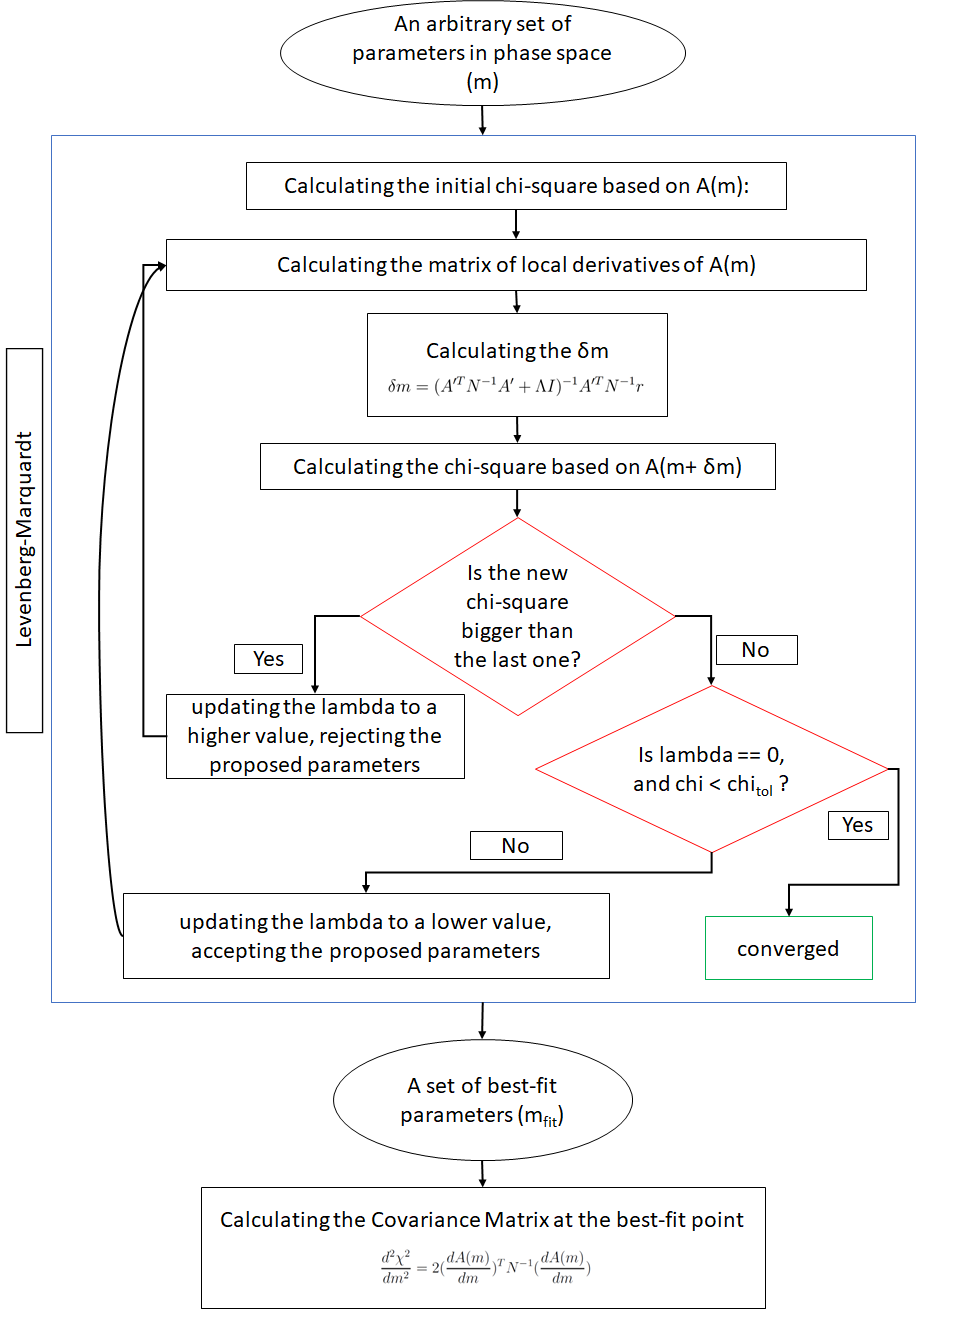
\includegraphics[scale =0.75]{LM_flow.png}
\caption[Flow chart of LM]{Flow chart depicting the Levenberg-Marquardt algorithm. The algorithm starts with the calculation of the $\chi^2$ based on the theoretical model predicted by the initial set of parameters. Then, the new new $\delta m$ is found using \ref{eq:LM} and its associated $\chi^2$ is calculated. The new $\chi^2$ is compared to its value from the last iteration and the value of the $\Lambda$ is determined upon the success or failure of the current iteration. The algorithm is considered as converged if $\Lambda = 0$ and the $\chi^2$ decreases less than a certain threshold amount.}
\label{fig:LM_flow}
\end{figure}
%--------------------------------------------------------------------------------
\section{Markov Chain Monte Carlo (MCMC)}
Given that Levenberg-Marquardt (LM) is not always effective in finding the best-fit point for complex likelihood spaces, a more powerful algorithm such as Markov Chain Monte Carlo (MCMC) is necessary in many real-life applications. \par
MCMC is particularly effective in fitting non-Gaussian likelihood spaces and has a guaranteed convergence, regardless of the starting point in parameter space. However, the algorithm is computationally heavy due to its iterative nature, which is based on the evaluation of chi-square on each step. Initially, an arbitrary point in parameter space is given to MCMC as its initial trial step and the associated chi-square is calculated. Then, a random point is drawn from a Gaussian distribution, where the mean is set at the last point in the chain\footnote{In Python applications, the numpy.randn function is used to serve this purpose.}. Subsequently, the new chi-square is compared to the previous one from the last trial step. If the new chi-square is lower, the new trial point is accepted in the chain. If the new chi-square is higher, the trial point is accepted with a probability determined by a specific criterion.\par
The above-mentioned probability threshold is typically defined as:
\begin{equation}
    Probability = e^{\frac{-1}{2}\left(\chi_{new}^2 - \chi^2\right)} 
    \label{eq:mcmc_probability}
\end{equation}
Which again has Gaussian insights.\par
As a measure of MCMC performance, the acceptance ratio is used to determine the fraction of trial steps that end up getting accepted into the chain. An ideal MCMC would typically have an acceptance ratio of 25 percent. However, even with a lower acceptance ratio, the MCMC can still converge, but it will require more trial steps.\par
A visual summary of MCMC algorithm is shown in \ref{fig:MCMC_flow}, and the Python code is available at \ref{chap:appendix,sub:MCMC}.
\begin{figure}[h!]
\centering
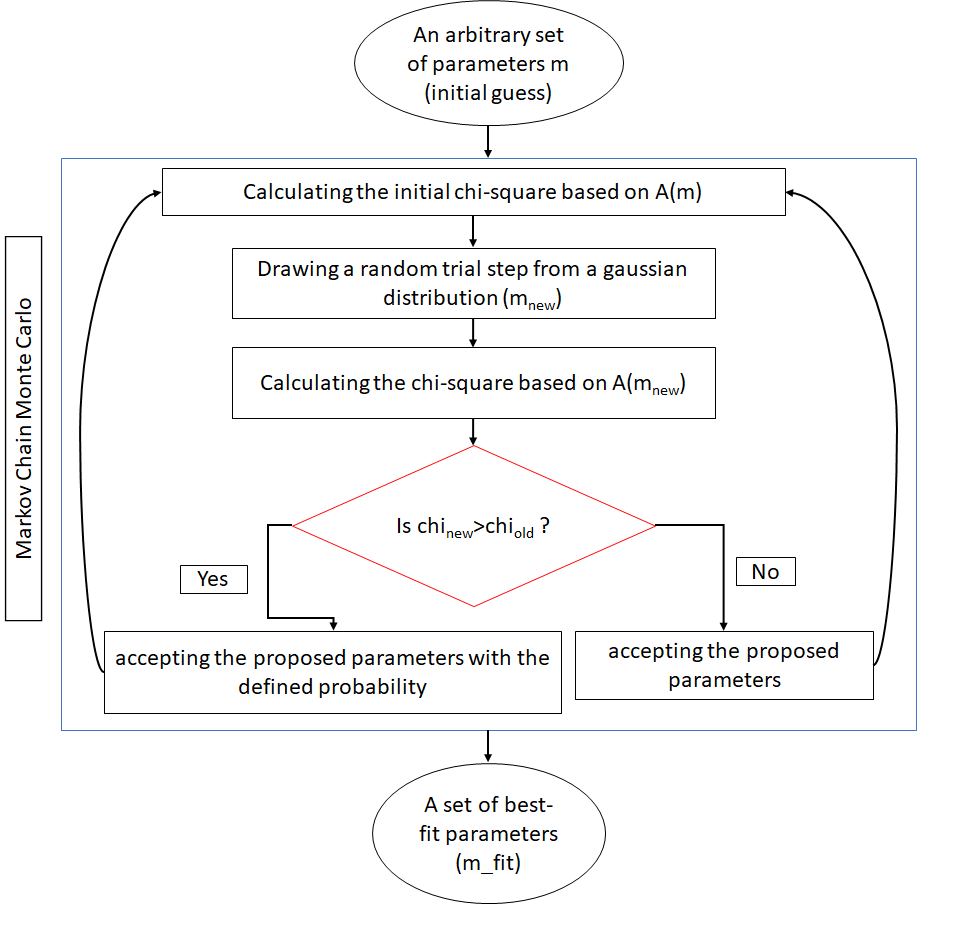
\includegraphics[scale =0.9]{MCMC_flow.png}
\caption[Flow chart of MCMC]{Flow chart depicting the Markov Chain Monte Carlo algorithm. The algorithm starts with the calculation of the $\chi^2$ based on the theoretical model predicted by the initial set of parameters. Then, a new set of parameters are drawn from independent one-dimensional gaussian distributions and the associated $\chi^2$ is calculated. The new $\chi^2$ is compared to its value from the last iteration. If $\chi^2$ has lowered, the new combination of parameters are accepted into the chain. Otherwise, the parameters will be accepted by the probability defined in \ref{eq:mcmc_probability}. The algorithm itself is not capable of testing its own convergence. Therefore, one needs to seek other approaches.}
\label{fig:MCMC_flow}
\end{figure}
%-----------------------------------------------------------------------------
\subsection{Convergence Test}
The MCMC algorithm is designed to explore different regions of the parameter space in order to reach convergence. Various methods have been developed to ensure that the MCMC has converged, one of which is to check the power spectrum.\par
The power spectrum represents the distribution of power at different frequencies in the MCMC chain. A converged MCMC chain must have the behaviour of a white noise, with power uniformly distributed among all frequencies. On the other hand, an unconverged chain will show more power at lower frequencies compared to higher ones. Therefore, the criterion for checking the convergence of an MCMC chain is the flatness of the power spectrum in low frequencies when plotted on a log-log scale. Figure \ref{fig:MCMC_unconverged} and \ref{fig:MCMC_converged} illustrates the difference between a converged and an unconverged chain.\par
\begin{figure}[h!]
\centering
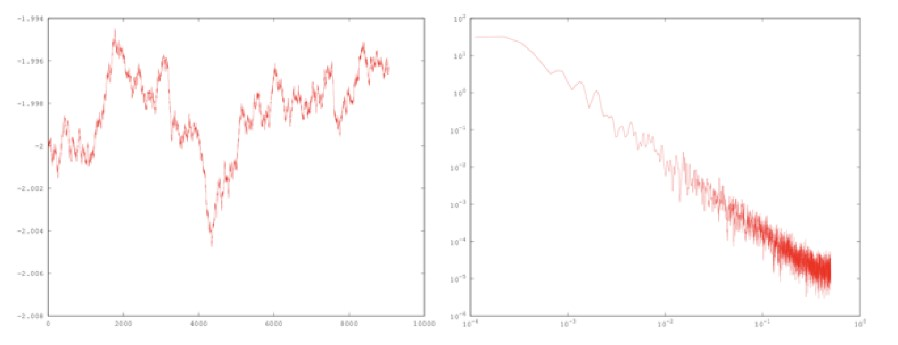
\includegraphics[scale =0.9]{mcmc_uncoverged.jpg}
\caption[An unconverged MCMC chain and its power spectrum]{An unconverged MCMC chain (left panel) and its power spectrum (right panel): A converged MCMC chain is expected to exhibit the behaviour of a white noise. Thus, on the power spectrum, the power shall be uniformly distributed among different frequencies (after the burn-in phase of the MCMC). Here, the power tends to increase in lower frequencies, and the chain itself does not indicate the behaviour of white noise. Therefore, this chain is not yet converged. Figure from Jonathan Sievers}
\label{fig:MCMC_unconverged}
\end{figure}

\begin{figure}[h!]
\centering
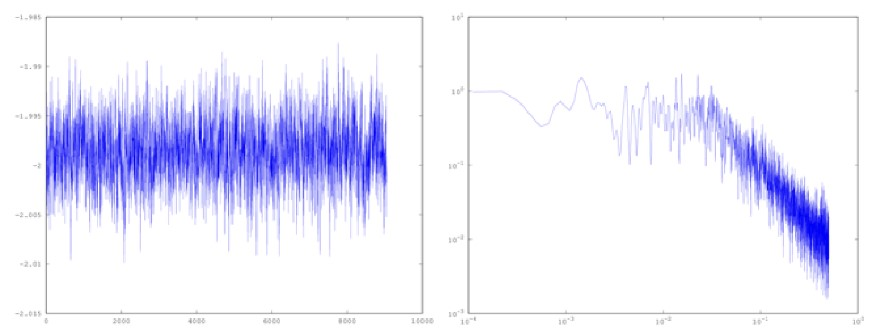
\includegraphics[scale =0.9]{mcmc_converged.jpg}
\caption[A converged MCMC chain and its power spectrum]{A converged MCMC chain (left panel) and its power spectrum (right panel): A converged MCMC chain is expected to exhibit the behaviour of a white noise. Thus, on the power spectrum, the power shall be uniformly distributed among different frequencies (after the burn-in phase of the MCMC). Here, the flat behaviour of the power spectrum is evident and the chain itself represents white noise. Figure from Jonathan Sievers}
\label{fig:MCMC_converged}
\end{figure}

%------------------------------------------------------------------------------------------------------
\section{Combination of MCMC and LM}
As mentioned before, MCMC is a computationally heavy algorithm due to its iterative nature. If calculating the chi-square takes a long time on each step, the MCMC itself will have a rather long run time before reaching the converged state. Different methods have been proposed to deal with this issue (\hl{citation}) and help the MCMC to converge faster, one of which is to use the insights from running LM \footnote{It worth to again mention that our sole rationale to use LM in our application is to generate a covariance matrix for the MCMC.}.\par
We previously discussed that parameters of a model might be correlated (\ref{chap:method,sub:cov_mat}). During a simple MCMC, we draw random samples from independent one-dimensional Gaussian distributions for each of the parameters. This samples do not take the possible correlations of parameters into account. On the other hand, generating samples using multivariate Gaussian distribution (joint normal distribution), will give us the capacity to encompass such characteristics. Eventually, the probability of them getting accepted into the actual chain will be higher. Eventually, we are able to summarize that this approach (feeding the MCMC with a posterior distribution) will eventually assist the MCMC to explore more efficient regions of parameter space, and converge faster. Figure \ref{fig:combined_flow} illustrates this technique briefly.\par
Since the covariance matrix of these needed samples is already in hand, we are able to easily generate a set of correlated noise samples from that. This procedure is described in the following section.\par

\begin{figure}[h!]
\centering
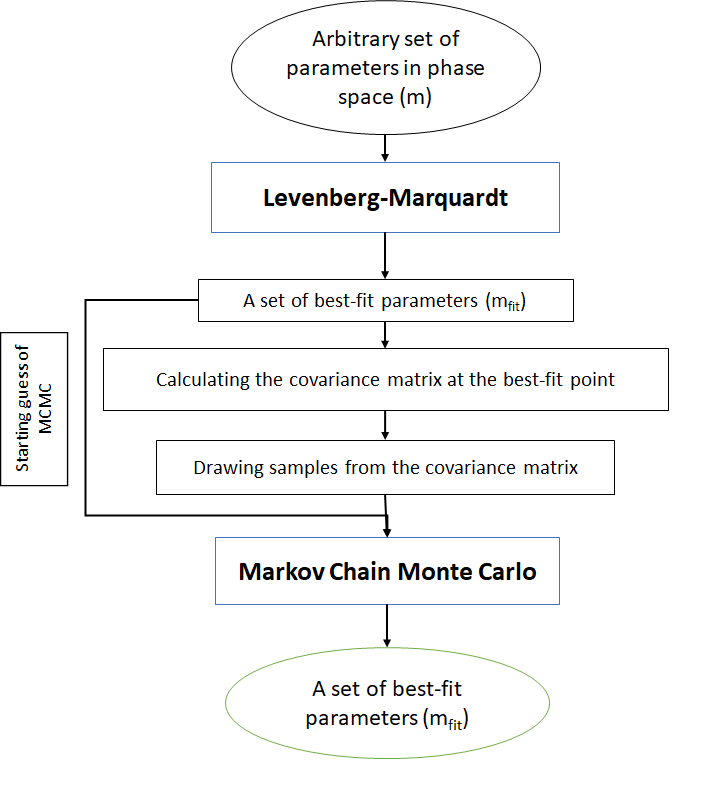
\includegraphics[scale =0.9]{combined_flow.png}
\caption[Flow chart of the procedure to combine MCMC and LM]{Flow chart of the procedure to combine MCMC and LM. We start by an arbitrary combination pf parameters in phase space and run the LM algorithm to find the best-fit point and the covariance matrix. Then, we draw sufficient samples from the covariance matrix to use them as the posterior distribution of our MCMC. Eventually, the output of this combined method is a set of best-fit parameters and their associated error bars.}
\label{fig:combined_flow}
\end{figure}

\subsection{Generating correlated noise}
\label{chap:method,sub:correlated noise}
As discussed before, the off-diagonal elements of a covariance matrix correspond to the inverse of covariance between each pair of parameters. Thus, if we draw samples from the inverse of covariance matrix (which needs to be calculated at the point of "best-fit"), we are essentially sampling from the multivariate normal distribution with the deviation values describing the uncertainties in the parameters\footnote{Figure \ref{fig:corner_plots}, which shows the corner plots for a four-variable gaussian model, emphasizes the importance of sampling from a multivariate normal distribution and taking the correlations between the parameters into account.}.\par
The equivalent methods can be used to generate correlated noise: Cholesky and eigenvalue decomposition\footnote{Normally, calculating the Cholesky decomposition takes a shorter amount of time.}. For practical reasons, we prefer to use the eigenvalue decomposition for 21cm applications. The procedure is a s follows: A matrix of normal gaussian-drawn random variables is constructed in the desired shape ($n \times m$, corresponding to the number of samples and number of parameters respectively). Then, it is multiplied by the eigenvalue matrix and scaled by the square root of the eigenvalues. The transpose of the product will give us the correlated samples. \par
To gain more precision, is it possible to use the eigenvalues decomposition of the normalized covariance matrix (where diagonal samples all equal unity). The normalization process is done by multiplying the covariance matrix with its own diagonal. Eventually, the drawn samples need to be scaled by the square root of the diagonal matrix.\par
The Python implementation of the above-mentioned procedure is given in \ref{chap:appendix,sub:draw}.

\begin{figure}[h!]
\centering
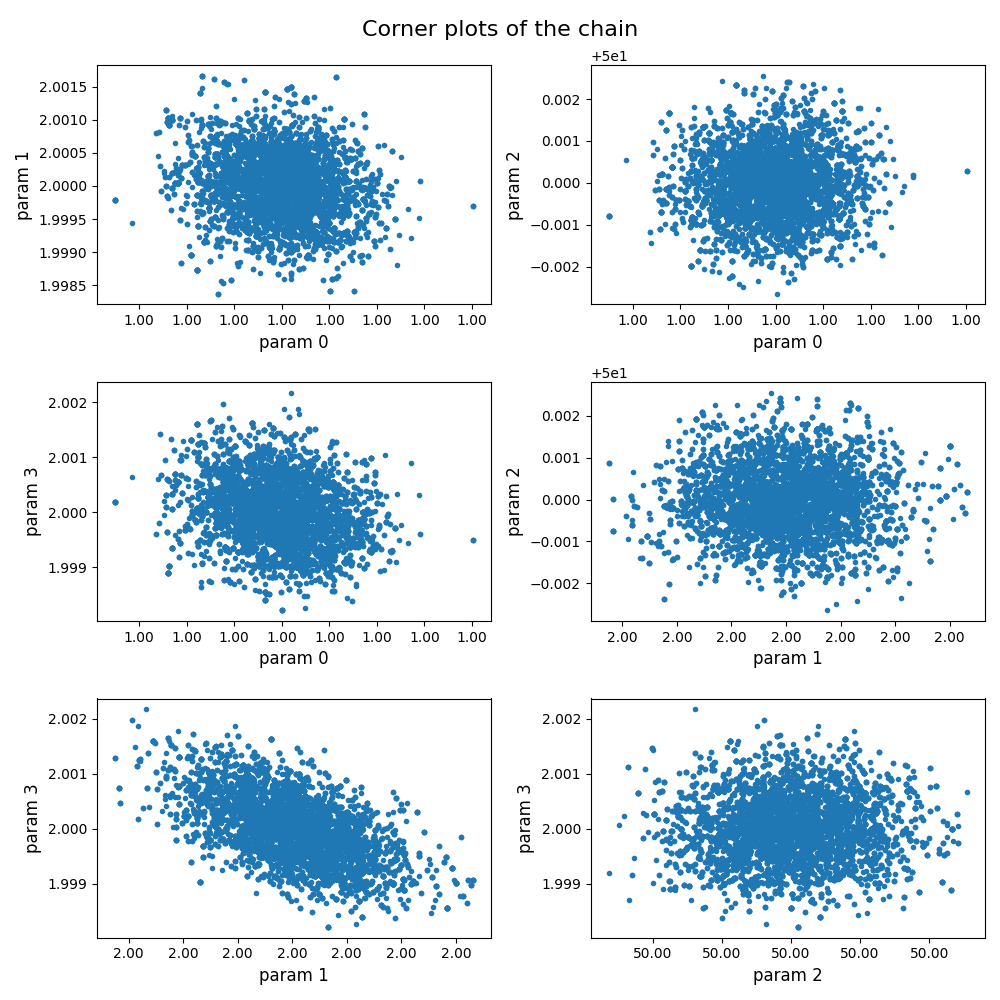
\includegraphics[scale =0.6]{corner_plot_chain.png}
\caption[Corner plots of an MCMC chain]{Corner plots (parameter vs parameter) of a typical MCMC chain from a four-variable Gaussian model. The lower right panel clearly shows patterns of correlation between a pair of parameters. Sampling from a multivariate normal distribution based on the covariance matrix associated with these samples will take the correlations into account.}
\label{fig:corner_plots}
\end{figure}

\section{Testing the Algorithm}
\label{chap:method,sub:test}
The complicated algorithm described in the previous sections, does not always behave as expected. Thus, naturally, one seeks options to weigh the output. In sections \ref{chap:method,sub:test,subsub:chi} and \ref{chap:method,sub:test,subsub:plot}, we introduce two methods to measure the overall quality of the model fitting.\par
\subsection{The chi-square test}
\label{chap:method,sub:test,subsub:chi}
This method is more focused on inspecting the output of LM and drawn samples. A large number of samples are drawn from the covariance matrix and the corresponding chi-squares are calculated. Since the covariance matrix describes the uncertainties in the parameters, we expect that the average difference in the chi-square statistics for two different samples should be of order unity per each parameter. This comes from the fact that the chi-square statistic scales with the uncertainties in the data and model, which are typically of order 1.\par
Figure \ref{fig:csq_test} shows an example of the distribution of difference between the chi-square values.\par
\begin{figure}[h!]
\centering
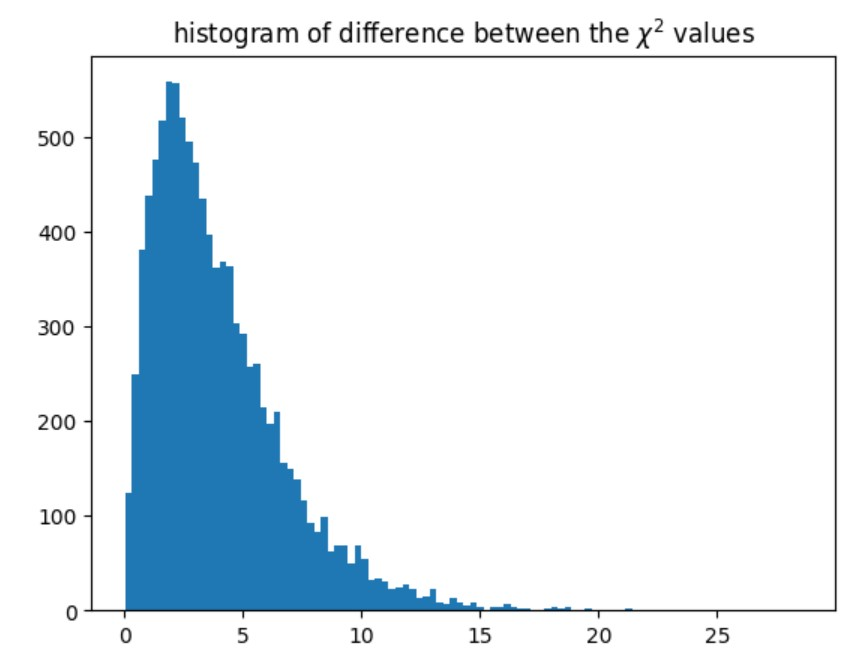
\includegraphics[scale =0.9]{chi-sqaure test.jpg}
\caption[Histogram of difference in the chi-square values of drawn samples]{Histogram illustrating the distribution of the values of difference between the chi-squares of drawn samples for a four variable Gaussian model. The samples are drawn from the covariance matrix calculated at the point of best-fit (output of LM). We expect the average difference in the $\chi^2$ statistics for two different samples to be of order unity per each parameter.
On this plot, the average of difference is 3.97 and the standard deviation is 2.83, in acceptable agreement with our expectations. Therefore, the best-fit parameters are considered as a "good fit".}
\label{fig:csq_test}
\end{figure}
\subsection{Chi-Square vs Parameters Plots}
\label{chap:method,sub:test,subsub:plot}
Another method to verify the results is to plot the chi-square values of drawn samples versus the each of the parameters. According to the definition of chi-square \ref{eq:chi-square matrix} (the non-linear dependency of chi-square on model parameters) we expect to observe a parabolic behaviour.\par
Figure \ref{fig:csq_params} demonstrates chi-square vs parameters plots for the same model as \ref{fig:csq_test}.
\begin{figure}[h!]
\centering
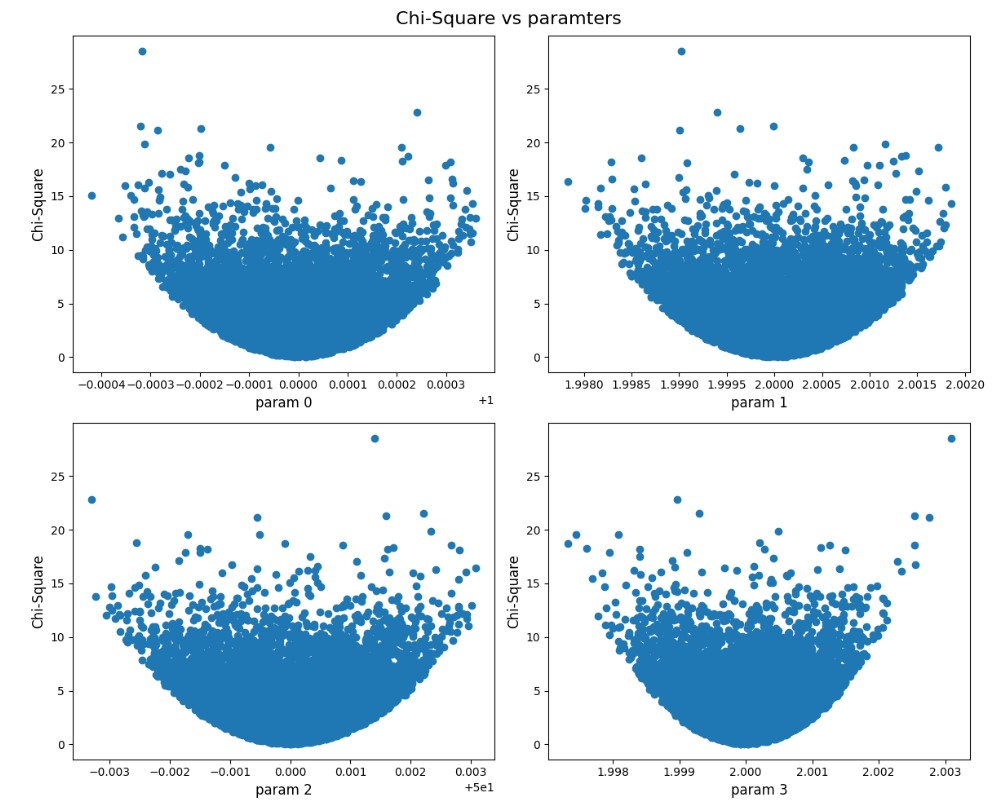
\includegraphics[scale =0.9]{csq_params.jpg}
\caption[Chi-Square vs parameters plots]{Figures demonstrating the values of chi-square associated with the drawn samples versus the values of parameters for a four variable Gaussian model. The $\chi^2$ is expected to have a parabolic dependency on the value of parameters based on its definition (\ref{eq:chi-square matrix}). This is a test to confirm the accuracy of covariance matrix and the procedure of sample drawing.}
\label{fig:csq_params}
\end{figure}
%###################################################################################
\chapter{Results and Analysis}
\label{chap:results}
Reminder: citations for physical explanation of parameters, I guess it is better to address pop\_rad\_yields with the physical meaning, but mention that the name is different in ARES documentary.\par
Chapter \ref{chap:method} carefully described a specific method to fit an experimental data set to its corresponding theoretical model. In this chapter, we are going to impose this method to actual global 21cm curves. We chose to use ARES as our simulator to generate these curves. \par

\section{Key Astrophysical Parameters in the Global 21cm Signal}
According to the discussed physics of the $21cm$ signal in section \ref{chap:global21cm,sub:physics}, the shape and amplitude of this signal are intensely dependent on underlying astrophysical processes, especially those related to the star formation and reheating of the IGM. In this section, we will take the discussion further and address our current understanding of this dependency on four specific parameters which are able to effectively span the global $21cm$.\par
By effectively constraining these parameters, significant progress can be made in comprehending the thermal history of the intergalactic medium (IGM) and the population of x-ray sources during high-redshift epochs \cite{21century}.\par

\begin{enumerate}
    \item \textbf{$f_X$}: High-redshift normalization factor in the relation between X-ray luminosity and SFR\\
    X-ray photons generated by galaxies and quasars are likely the most important cause of heating the IGM. Considering the fact that the nature of high-redshift objects are not very well identified, it is not possible to give an exact theory for the high-redshift X-ray background. The safest course of action is to assume that the correlation between X-ray luminosity and SFR in high redshift is only an extrapolation of its local format.
    \begin{equation}
        L_X = 3.4 \times 10^{40} f_X \left( \frac{SFR}{1 \hspace{0.1cm} M_{\odot} \hspace{0.1cm} yr^{-1}}\right) \hspace{0.1cm} erg \hspace{0.1cm}s^{-1}
    \end{equation}
    Where $f_X$ is an unknown normalization factor at high redshift and is believed to evolve by redshift. The normalization was chosen so that, with $f_X =1$, the total X-ray luminosity per unit SFR is consistent with that observed in starburst galaxies at the present epoch \cite{low_frequency, 21century}.
    
    \item \textbf{$N_{lw}$}: Number of photons emitted in the Lyman-Werner band ($11.2-13.6eV$) per baryon of star formation (This parameter is referred to as \emph{pop\_rad\_yield\_0\_} in ARES documentation), cite ARES documentation\\ read the relevant section on this paper \cite{lw_background}
    
    \item \textbf{$N_{ion}$}: Mean number of ionizing photons produced per baryon of star formation (This parameter is referred to as \emph{pop\_rad\_yield\_2\_} in ARES documentation)
    
    \item \textbf{$f_{esc}$}: Fraction of ionizing photons that escape their host galaxy into the IGM\\
    $f_{esc}$ and $N_{ion}$ are both defined in the process of calculating the evolution of ionization fraction $\bar{x}_i$:
    \begin{gather}
        \bar{x}_i = \frac{\zeta f_{coll}}{1 + \bar{n}_{rec}}\\
        f_{coll} = \int_{m_{min}}^\infty dm \hspace{0.1cm} m \hspace{0.1cm} n\left(m\right)\\
        \zeta = A_{He} \hspace{0.1cm} f_* \hspace{0.1cm} f_{esc} \hspace{0.1cm} N_{ion}
    \end{gather}
    
    $f_{coll}$ is the collapse fraction (fraction of gas inside collapsed objects, fraction of mass in halos more massive than $m_{min})$, $\bar{n}_{rec}$ is the mean number of recombinations per ionized hydrogen atom, $\zeta$ is the ionizing efficiency, $f_*$ is the star formation efficiency (fraction of baryons converted into stars), and $A_{He} = 4/(4 - 3Y_p) = 1.22$, where $Y_p$ is the mass fraction
    of helium, is a correction factor to convert the number of ionizing photons per baryon in stars to the fraction of ionized hydrogen. Our limited understanding of the mass distribution of the emitting stars introduces an uncertainty in the number of ionizing photons per baryon $N_{ion}$ that is emitted by galaxies. There is also considerable uncertainty in the fraction of ionizing photons $f_{esc}$ that escape the host galaxy to ionize the IGM. That's why we chose these parameters. Observations will help to constrain them.\\
    These parameters enter our model as a factor multiplying the SFR and are, therefore, individually degenerate with the star-formation efficiency $f_*$. That's why we did not choose to use $f_*$  \cite{low_frequency, 21century}.
\end{enumerate}
Figure \ref{fig:sensivity} shows the effect of changing these parameters on an actual 21cm curve.\par

We take the above-mentioned physical parameters as fitting parameters and we try to find their best-fit values and corresponding error-bars.\par
%-----------------------------------------------------------------------------------
\section{Parameter Estimation of an ARES generated curve}
\label{chap:results,sub:known_curve}
Before using our developed script to fit actual data, we use it to fit a known ARES curve as a verification test. We generate an ARES curve with a fixed set of parameters and we use these curve as the imaginary "data". If the algorithm returns the same parameter values (with in the error-bar range), we can make sure that it is working correctly.\par
We begin by using the LM and we find inverse of covariance matrix for our chosen combination of parameters, which we will later use to generate our correlated samples.\par
Parameters:
\begin{equation}
\emph{pop\_rad\_yield\_0\_}: 10^4, \quad \emph{pop\_rad\_yield\_2\_}: 10^3,\quad f_{esc}: 0.1,\quad f_X: 0.1 
\label{eq:parameter_values}
\end{equation}
Inverse of covariance matrix for this set of parameters:
\begin{equation}
\label{eq:cov_mat_known_curve}
    \begin{pmatrix}
    1.64\times 10^{-3} & 1.96 \times 10^{-2} &  -4.39 \times 10^{-7} &  -5.37 \times 10^{-8} \\
    1.96 \times 10^{-2} &  1.60 \times 10^{1} &  -1.44 \times 10^{-3} &  -5.94 \times 10^{-6} \\
    -4.39 \times 10^{-7} &  -1.44 \times 10^{-3} &  1.38 \times 10^{-7} &  2.15 \times 10^{-10} \\
    -5.37 \times 10^{-8} &  -5.94 \times 10^{-6} &  2.15 \times 10^{-10} &  1.38 \times 10^{-11} 
    \end{pmatrix}
\end{equation}
Now, we are prepared to draws our samples based on method described in \ref{chap:method,sub:correlated noise}. Figure \ref{fig:histogram_samples_known_curve} illustrates the distribution of samples for the above-mentioned four parameters. As a sanity check, we calculate the mean and standard deviation of these distribution. We expect the mean to be close to values of \ref{eq:parameter_values}. Table \ref{tab:samples_mean_known_curve} represents the values of mean and standard deviation, which is in agreement with the expectations.\par

\begin{table}
\centering
\caption[Mean and standard deviation of samples]{Mean and standard deviation of samples drawn from the covariance matrix \ref{eq:cov_mat_known_curve}}
\label{tab:samples_mean_known_curve}
\begin{tabular}{|c|c|c|c|c|}
\hline
\diagbox{Value}{Parameter} & \emph{pop\_rad\_yield\_0\_} & \emph{pop\_rad\_yield\_2\_} & \emph{$f_{esc}$} & \emph{$f_X$}\\
\hline
Mean & $9.99999993 \times 10^{3}$ & $1.00002933 \times 10^{3}$ & $9.99962873 \times 10^{2}$ & $1.00000029 \times 10^{1}$\\
\hline
Standard Deviation & $4.08174690 \times 10^{2}$ & $4.03138658 \times 10^{0}$ & $3.74407952 \times 10^{4}$ & $3.72581029 \times 10^{6}$\\
\hline
\end{tabular}
\end{table}


In section \ref{chap:method,sub:test}, we introduced two methods to check the algorithm and the quality of fit. Performing the chi-square test on our samples showed that the average difference between the chi-square of drawn samples is 49.20, which we expected to be ~4. Although it is approximately one order of magnitude bigger that the expectations, it can be still considered a good fit.\par

We proceed by performing the second test, which is plotting the values of ch-square of samples versus the parameter values. The results are shown in \ref{fig:csq_hist_known_curve}. In the hypothetical ideal case, We expected to see a parabolic behaviour. Figure \ref{fig:csq_vs_params_zoomed_known_curve} shows the zoomed version of results. We can infer a parabolic behaviour in low values of chi-square.\par

Now that we have our samples, we proceed to run the MCMC chain with them. The overall results of the fit and the final resulting curve are shown in \ref{tab:mcmc_results_known_curve} and \ref{} respectively.
Figure \ref{fig:chain_known_curve} indicates the white-noise behaviour of parameters throughout the chain which is consistent with our anticipation for a converged chain. We confirm the convergence by looking at the power spectrum in Figure \ref{fig:power_spectrum_known_curve}. Flat behaviour in low frequencies is apparent.\par


\begin{table}
\centering
\caption[Results of fitting a known ARES curve with MCMC chain]{Results of fitting a known ARES curve with MCMC chain}
\label{tab:mcmc_results_known_curve}
\begin{tabular}{|c|c|c|c|c|}
\hline
\diagbox{Value}{Parameter} & \emph{pop\_rad\_yield\_0\_} & \emph{pop\_rad\_yield\_2\_} & \emph{$f_{esc}$} & \emph{$f_X$}\\
\hline
True values & $1 \times 10^ {4}$ & $1 \times 10^ {3}$ & 0.1 & 0.1\\
\hline
Fitted values & $9.99998275 \times 10^ {3}$ & $9.99419824 \times 10^ {2}$ & $1.00025031 \times 10^ {-1}$ & $1.00001169 \times 10^ {-1}$ \\
\hline
Error-bar of fit & $3.54171104 \times 10^ {-2}$ & $3.86126208 \times 10^ {0}$& $3.57822431 \times 10^ {-4}$ & $3.39295495 \times 10^ {-6}$ \\
\hline
Fitting Error & 0.00013093\% & 0.02645403 \%& 0.01527014\%& 0.00032365\%\\
\hline
\end{tabular}
\end{table}
\hl{It is worth mentioning that the method described in chapter \ref{chap:method} and used in this section, is flexible to the change of parameters of the model (which in our case, is ARES.\footnote{List of parameters can be found in \hyperlink{https://ares.readthedocs.io/en/latest/}{ARES documentation}.}). However, these parameters are only physically meaningful in a limited region of phase space (A hypercube where the combination of parameters are physically meaningful). Going beyond this region will result in a failure in calculating the global 21cm curve. our developed script is designed to handle this issue and stop it from aborting the whole run \footnote{The python code for the MCMC is designed such that it will return an arbitrary large chi-square for those combination of parameters which ARES is unable to handle. Therefore, the probability of these points getting accepted into the chain will be systematically low.}, but the MCMC might not be able to reach convergence if the algorithm faces a lot of samples beyond the allowed region.}\par
%-----------------------------------------------------------------------------------
\section{Parameter estimates of EDGES data and uncertainties}
\subsection{Choice of "multiplication factor"}
\subsection{error bar calculation}
Reminder: not exactly sure where this equation comes from\par

We need to know the error bar of the observational data (EDGES) to run the MCMC chain. These error bars are usually taken from the noise model. In order to make our life easy, instead of dealing with the EDGES noise model which is hard and messy, we use the following straight forward equation which comes from the radiometer equation:\par
\begin{equation}
    \frac{\delta T}{T_{sys}} = \frac{1}{\sqrt{Bt}}
\end{equation}
Where B is the bandwidth, t is the exposure time and $T_{sys}$ is the system temperature. Assuming the bandwidth of $10^6$, exposure time of one day and and temperature of 3000K, we get:
$\delta T = 10 ^{-2}K = 10mK$
\subsection{results}
We proceed by doing the same procedure as section \ref{chap:results,sub:known_curve}. However, this time we use the EDGES data (with half of the actual amplitude) as our observational data in MCMC. This half amplitude is chosen using the insights from section \ref{chap:results,sub:m_factor}. One of the main issues is that since the shape of the EDGES data is not very close to the predicted theoretical curve, the resulting fit is not very perfect. We first run the LM to find the covariance matrix and generate our samples. 
\begin{equation}
\label{eq:cov_mat_edges}
    \begin{pmatrix}
    3.24\times 10^{4} & 5.68 \times 10^{6} &  -8.51 \times 10^{2} &  5.65 \times 10^{-1} \\
    5.68 \times 10^{6} &  2.43 \times 10^{10} &  -3.63 \times 10^{6} &  5.64 \times 10^{0} \\
    -8.51 \times 10^{2} &  -3.63 \times 10^{6} &  5.44 \times 10^{2} &  -9.80 \times 10^{-4} \\
    5.65 \times 10^{-1} &  5.64\times 10^{00} &  -9.80\times 10^{-4} &  3.92 \times 10^{-5} 
    \end{pmatrix}
\end{equation}

\begin{table}
\centering
\caption[Mean and standard deviation of samples]{Mean and standard deviation of samples drawn from the covariance matrix \ref{eq:cov_mat_edges}}
\label{tab:samples_edges}
\begin{tabular}{|c|c|c|c|c|}
\hline
\diagbox{Value}{Parameter} & \emph{pop\_rad\_yield\_0\_} & \emph{pop\_rad\_yield\_2\_} & \emph{$f_{esc}$} & \emph{$f_X$}\\
\hline
Mean & $4.54933238 \times 10^{3}$ & $2.47654876 \times 10^{3}$ & $3.70006283 \times 10^{-1}$ & $1.36397845 \times 10^{-1}$\\

\hline
Standard Deviation & $1.81616137 \times 10^{-1}$ & $1.56788160 \times 10^{2}$ & $2.34431702 \times 10^{-2}$ & $6.32705006 \times 10^{-6}$\\

\hline
\end{tabular}
\end{table}
We again run the MCMC from the drawn samples. The results are shown in table \ref{tab:mcmc_results_known_curve}. Figure \ref{fig:csq_trend_knwon_curve} and \ref{fig:corner_plots_known_curve} present the trend of values of chi-square throughout the chain and corner plots of parameters.Figure \ref{fig:csq_trend_knwon_curve} and \ref{fig:corner_plots_known_curve} present the trend of values of chi-square throughout the chain and corner plots of parameters.\par

\begin{table}
\centering
\caption[Results of fitting EDGES data with MCMC chain]{Results of fitting EDGES data with MCMC chain}
\label{tab:mcmc_results_known_curve}
\begin{tabular}{|c|c|c|c|c|}
\hline
\diagbox{Value}{Parameter} & \emph{pop\_rad\_yield\_0\_} & \emph{pop\_rad\_yield\_2\_} & \emph{$f_{esc}$} & \emph{$f_X$}\\
\hline
Fitted values & $9.999 \times 10^ {3}$ & $9.994 \times 10^ {2}$ & $1.000 \times 10^ {-1}$ & $1.000 \times 10^ {-1}$ \\
\hline
Error-bar of fit & $3.541 \times 10^ {-2}$ & $3.861 \times 10^ {0}$& $3.578 \times 10^ {-4}$ & $3.392\times 10^ {-6}$ \\
\hline
\end{tabular}
\end{table}
% -------------------------------------------------------------------------------------
\begin{figure}[h!]
\centering
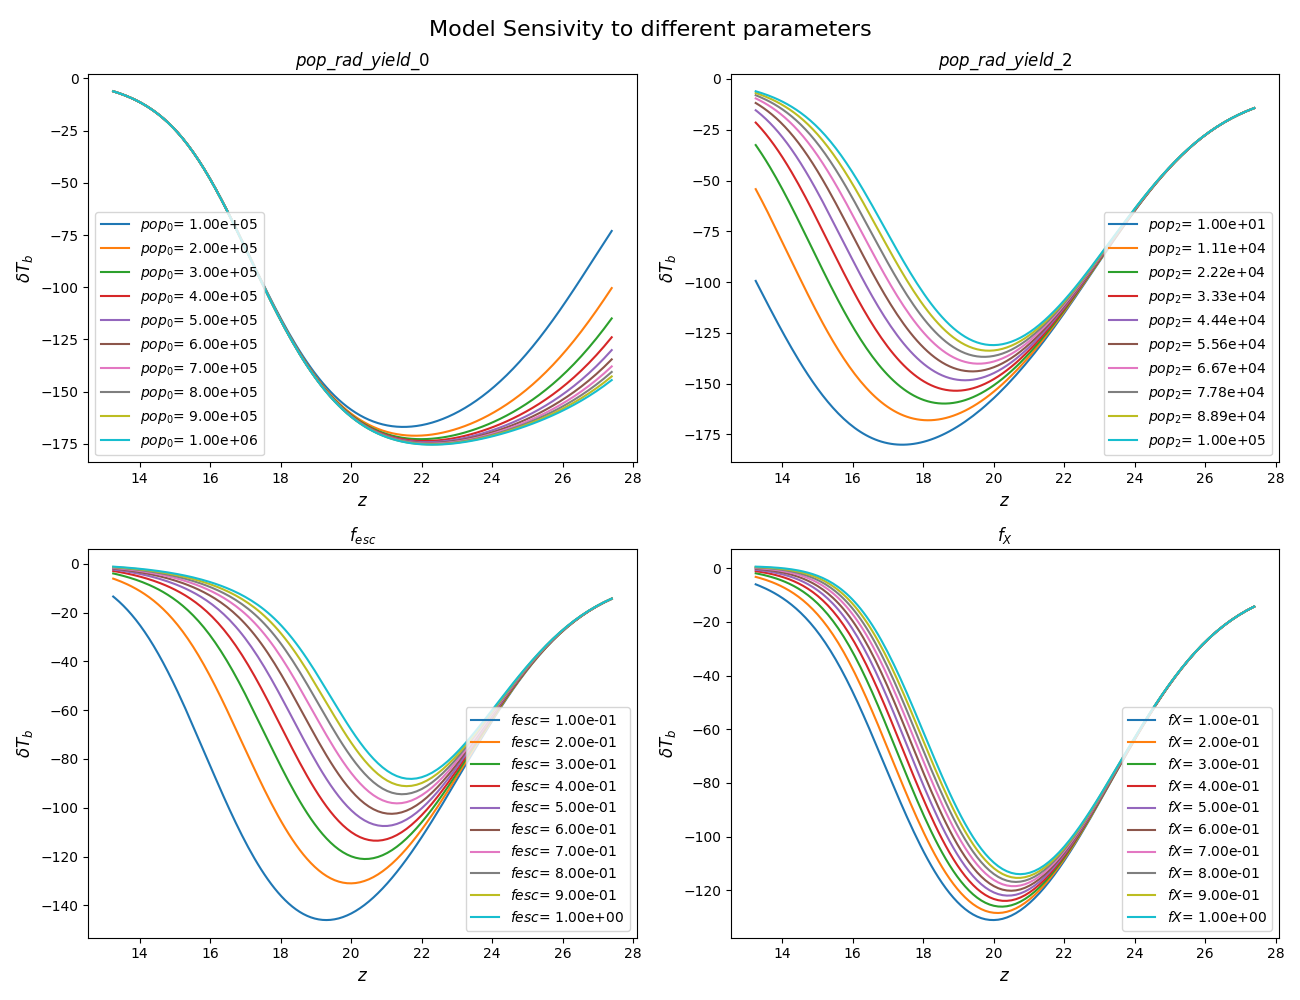
\includegraphics[scale =0.5]{sensivity.png}
\caption[Behaviour of global 21cm model with respect to chosen parameters]{Behaviour of ARES-generated global 21cm models with respect to four parameters: \emph{pop\_rad\_yield\_0\_}, \emph{pop\_rad\_yield\_2\_}, $f_{esc}$, and $f_X$. In each panel, the corresponding parameter posses 10 different values and all other parameters are kept at default values by ARES}
\label{fig:sensivity}
\end{figure}

\begin{figure}[h!]
\centering
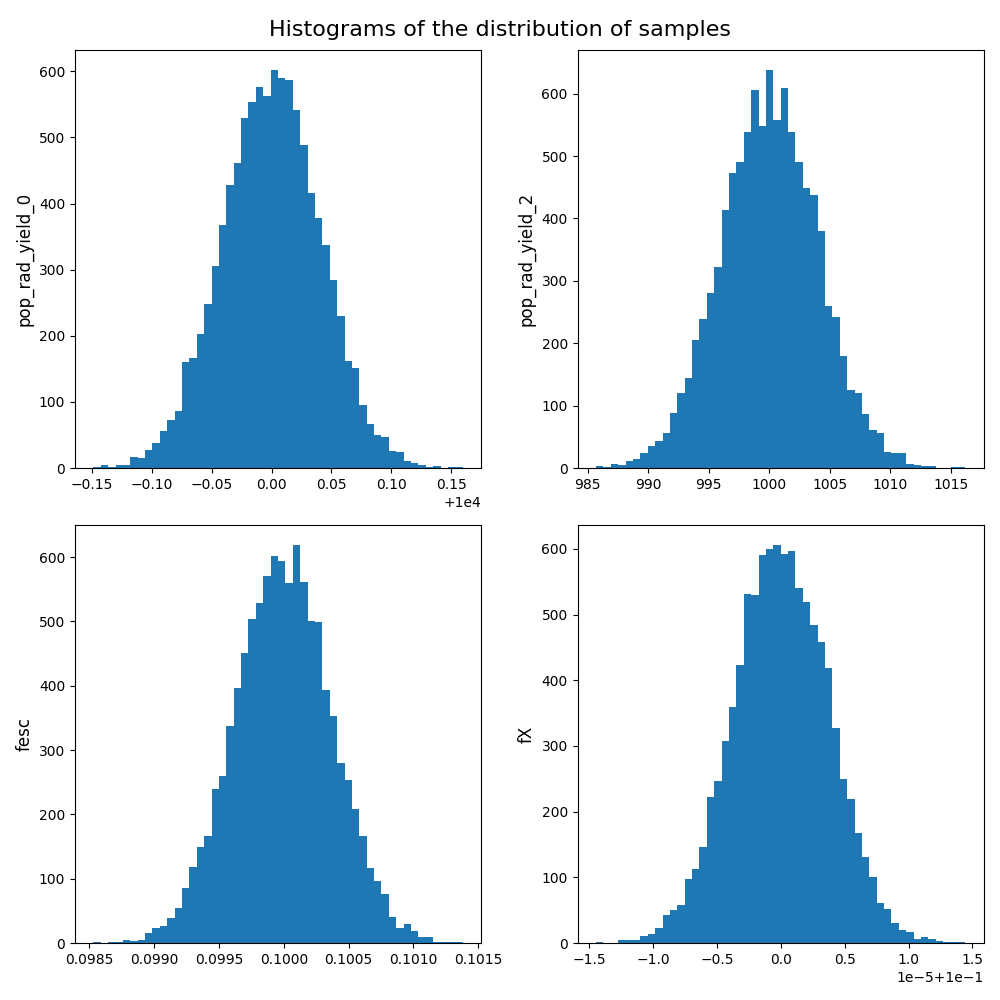
\includegraphics[scale =0.5]{histograms_known_curve.png}
\caption[Histogram of distribution of samples]{Histogram of distribution of samples before feeding to MCMC, The mean of these distributions are consistent with values given in \ref{eq:parameter_values}.}
\label{fig:histogram_samples_known_curve}
\end{figure}

\begin{figure}[h!]
\centering
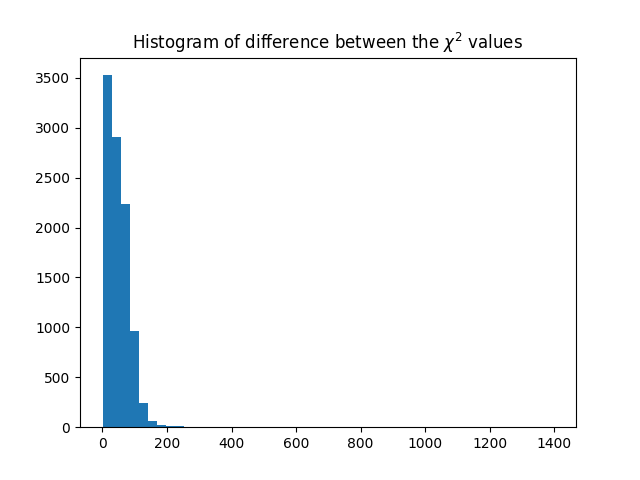
\includegraphics[scale =0.7]{csq_hist_known_curve.png}
\caption[Histogram of Chi-Square of drawn samples]{Histogram of Chi-Square of drawn samples, the mean is 49.20 with standard deviation of 41.98.}
\label{fig:csq_hist_known_curve}
\end{figure}

\begin{figure}[h!]
\centering
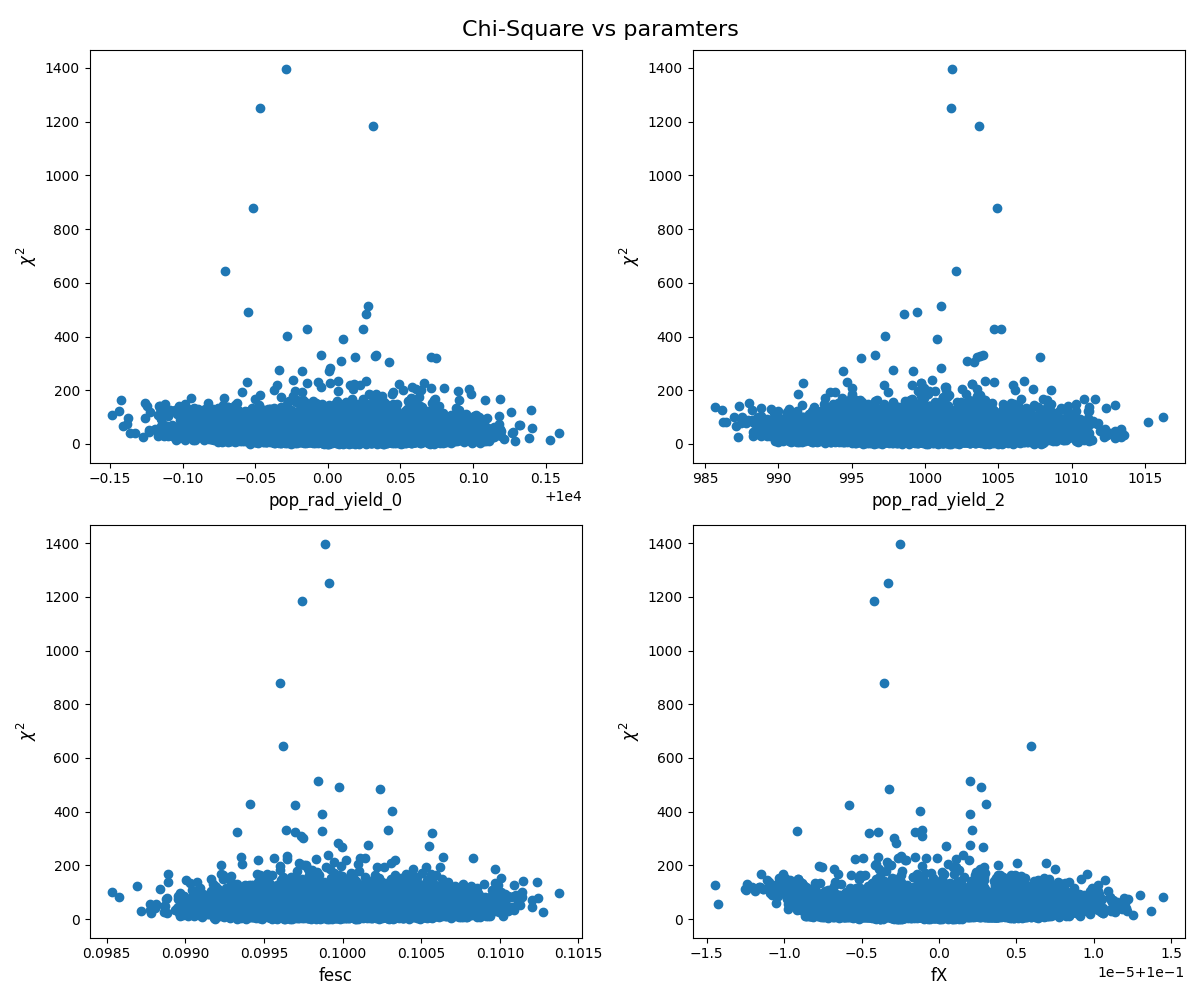
\includegraphics[scale =0.5]{csq_vs_params_knwon_curve.png}
\caption[Chi-Square of Drawn samples vs parameter values]{Chi-Square of Drawn samples versus parameter values for a known ARES curve with four parameters, The parabolic behaviour is not obvious in these plots.}
\label{fig:csq_vs_params_knwon_curve}
\end{figure}

\begin{figure}[h!]
\centering
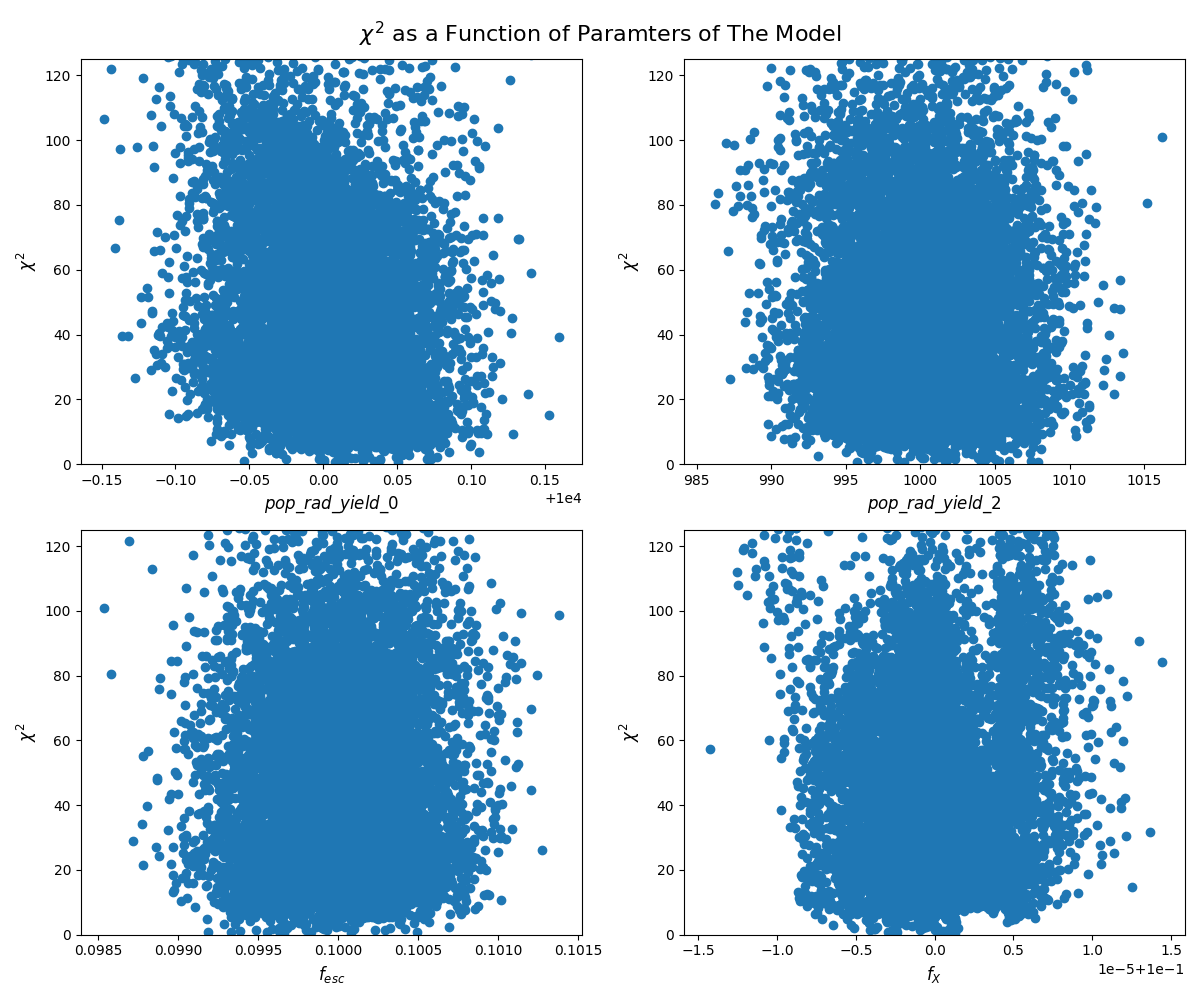
\includegraphics[scale =0.5]{csq_vs_params_zoomed_known_curve.png}
\caption[Chi-Square of Drawn samples vs parameter values, zoomed]{Zoomed version of figure \ref{fig:csq_vs_params_knwon_curve}, A weak parabolic behaviour is observed for low values of $\chi^2$.}
\label{fig:csq_vs_params_zoomed_known_curve}
\end{figure}

\begin{figure}[h!]
\centering
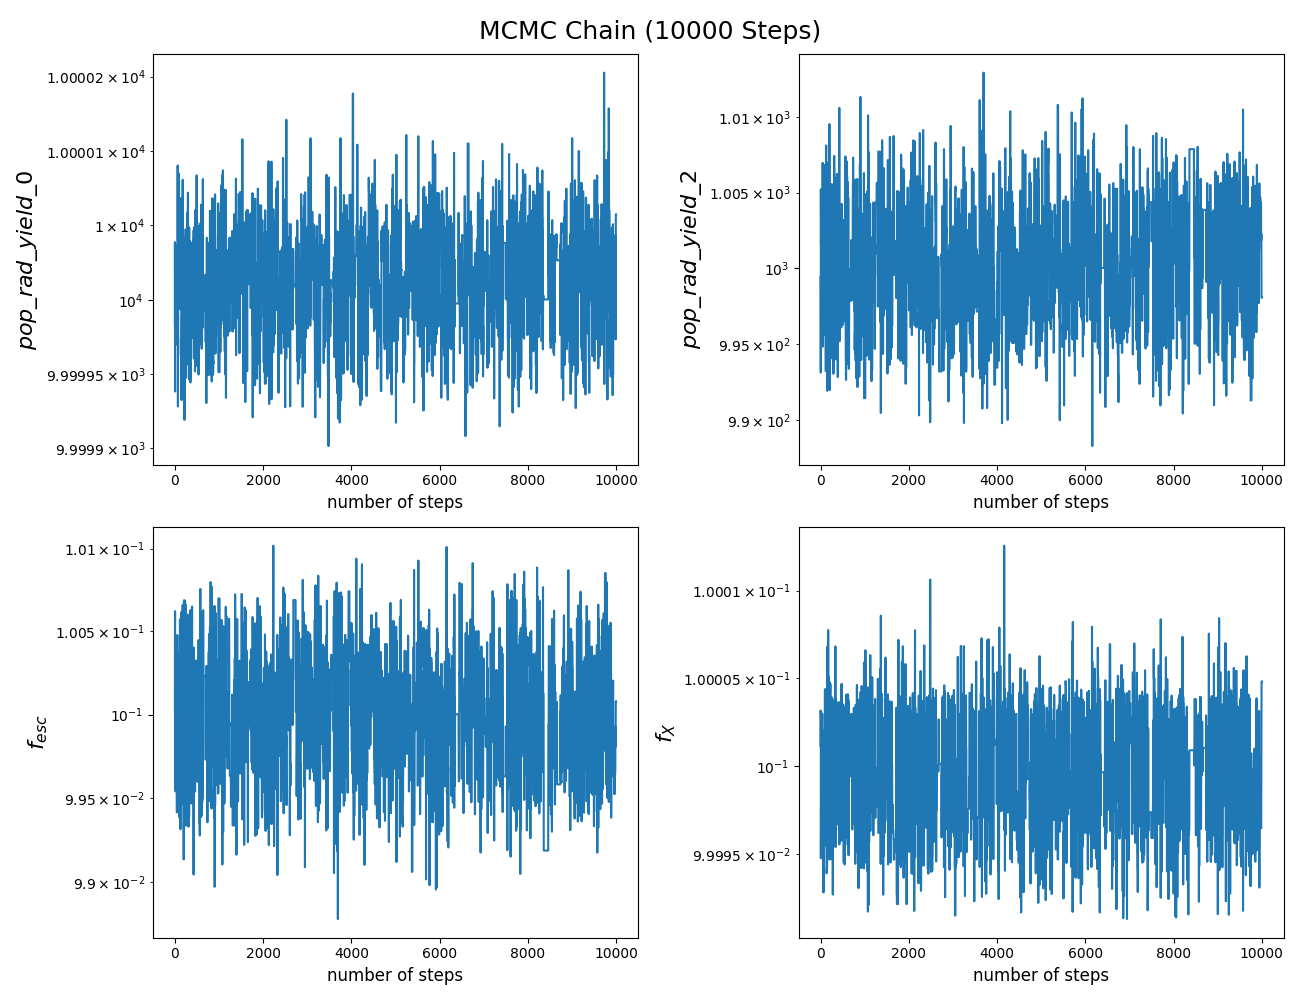
\includegraphics[scale =0.5]{chain_known_curve.png}
\caption[Trend of parameters]{Trend of parameters in the MCMC chain, White noise behaviour is considered as a sign of convergence. The acceptance ratio of the chain is $22.12\%.$}
\label{fig:chain_known_curve}
\end{figure}

\begin{figure}[h!]
\centering
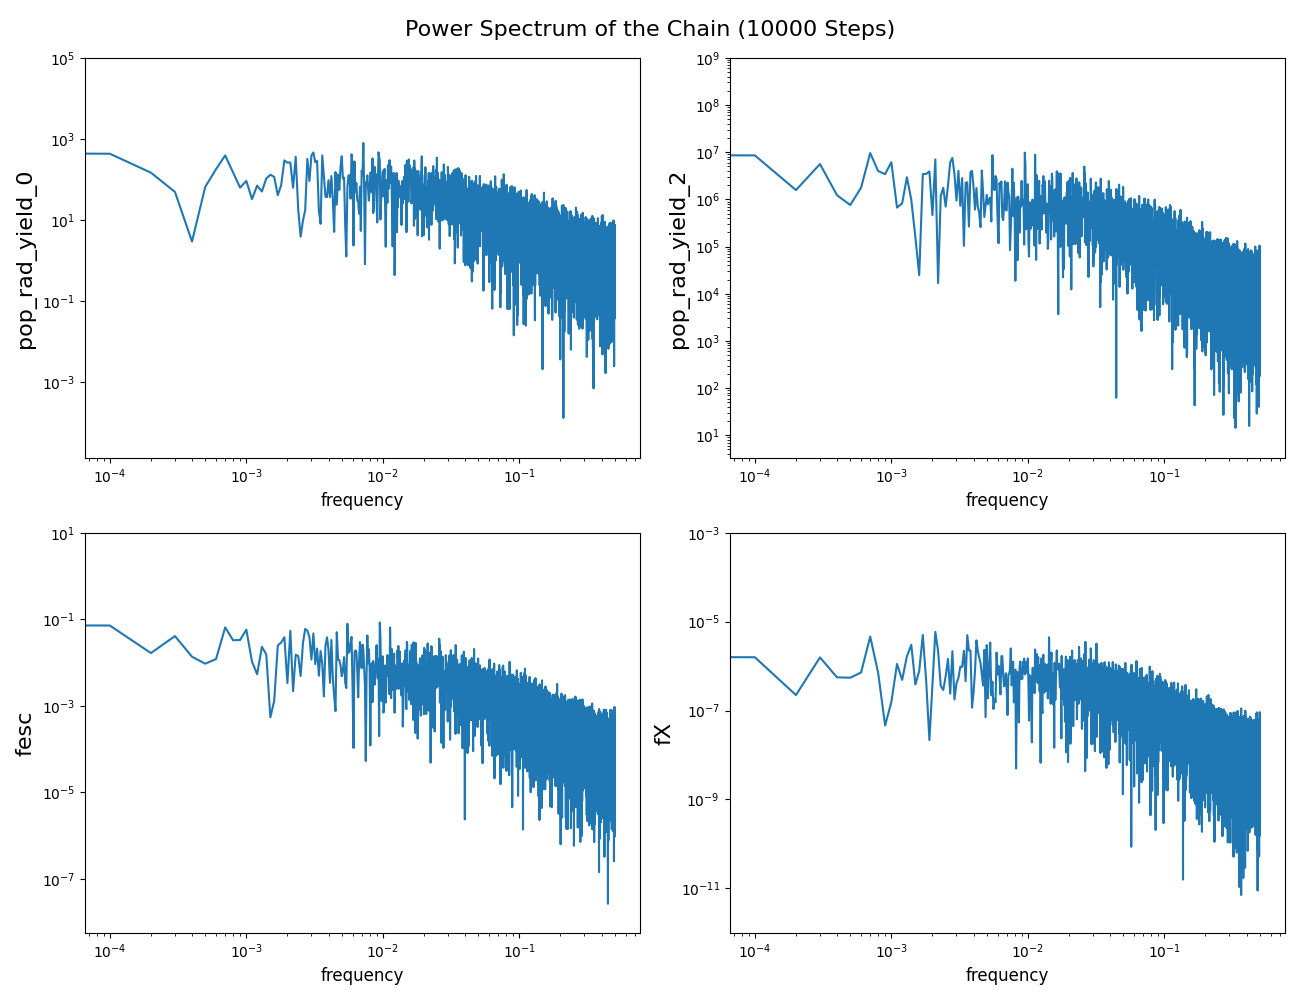
\includegraphics[scale =0.5]{power_spectrum_known_curve.png}
\caption[Power spectrum of the chain]{Power spectrum of the chain, Flat behaviour in low frequencies is in agreement with results of \ref{fig:chain_known_curve}.}
\label{fig:power_spectrum_known_curve}
\end{figure}

\begin{figure}[h!]
\centering
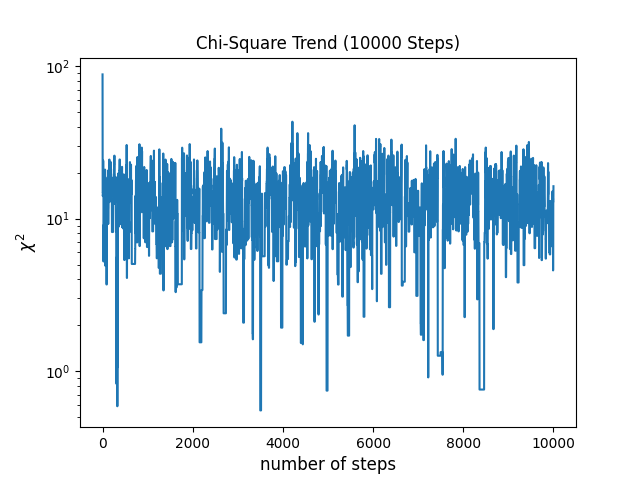
\includegraphics[scale =0.6]{csq_trend_knwon_curve.png}
\caption[Trend of chi-square]{Trend of chi-square in the MCMC chain, The chain seems to have reached an equilibrium state.}
\label{fig:csq_trend_knwon_curve}
\end{figure}

\begin{figure}[h!]
\centering
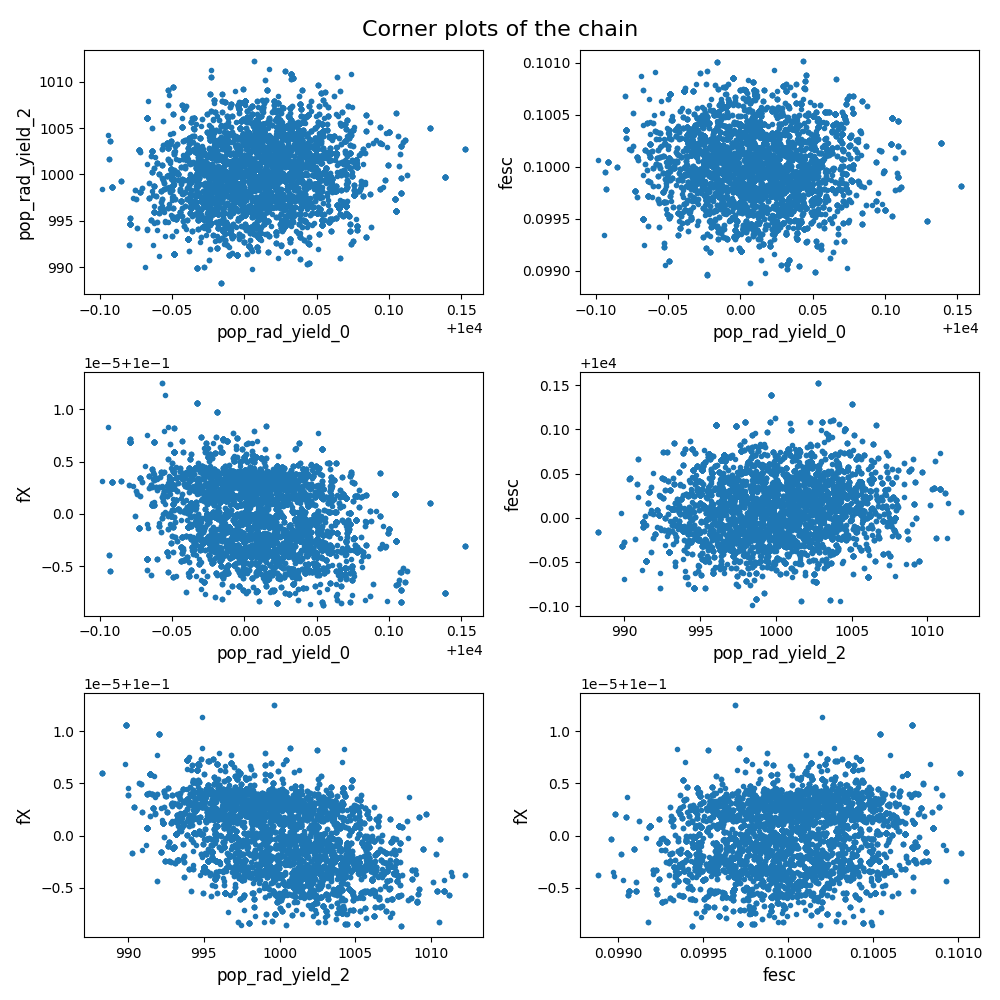
\includegraphics[scale =0.6]{corner_plots_known_curve.png}
\caption[Corner plots of the chain]{Corner plots of the chain indicating the correlation between the parameters specially in the lower left panel}
\label{fig:corner_plots_known_curve}
\end{figure}
%@@@@@@@@@@@@@@@@@@@@@@@@@@@@@@@@@@@@@@@@@@@@@@@@@@@@@@@@@@@@@@@@@@@@@@@@@@
\begin{figure}[h!]
\centering
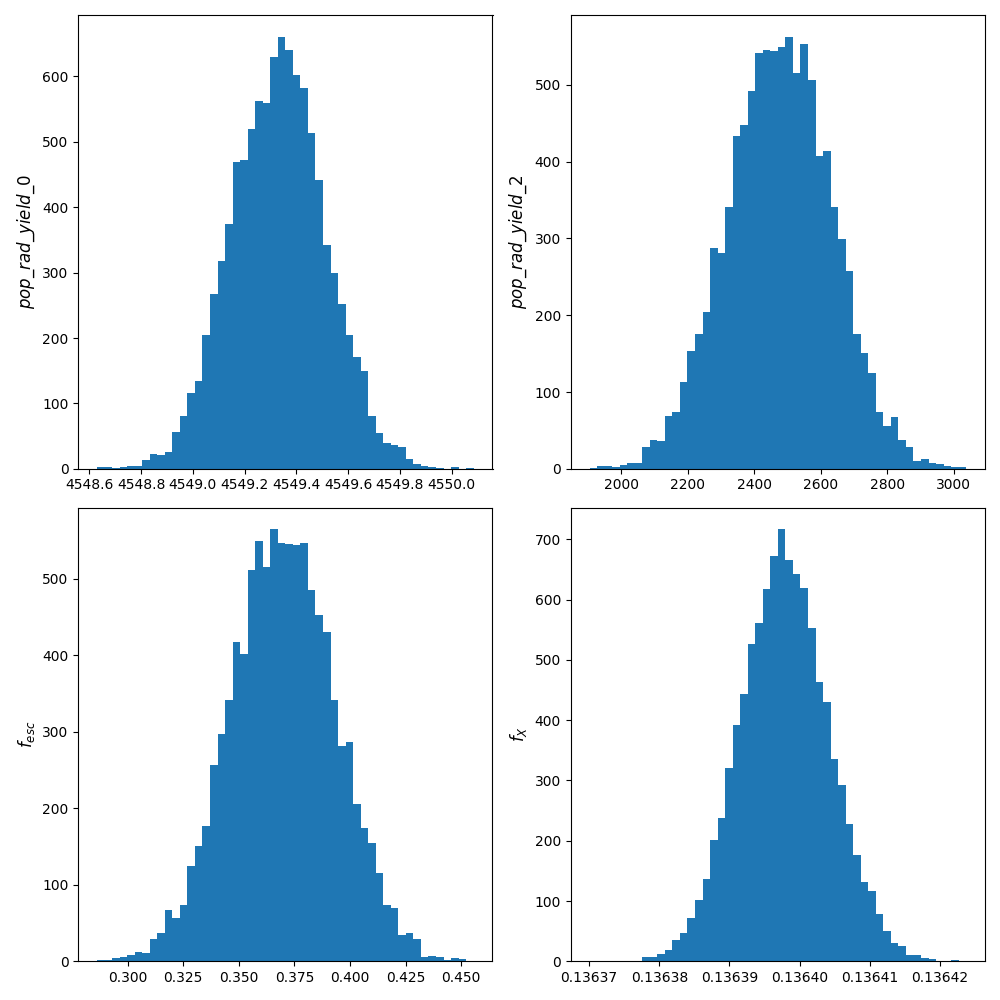
\includegraphics[scale =0.5]{histograms_edges.png}
\caption[Histogram of distribution of samples]{Histogram of distribution of samples before feeding to MCMC, The mean of these distributions are consistent with values given in \ref{eq:parameter_values}.}
\label{fig:histogram_samples_known_curve}
\end{figure}

\begin{figure}[h!]
\centering
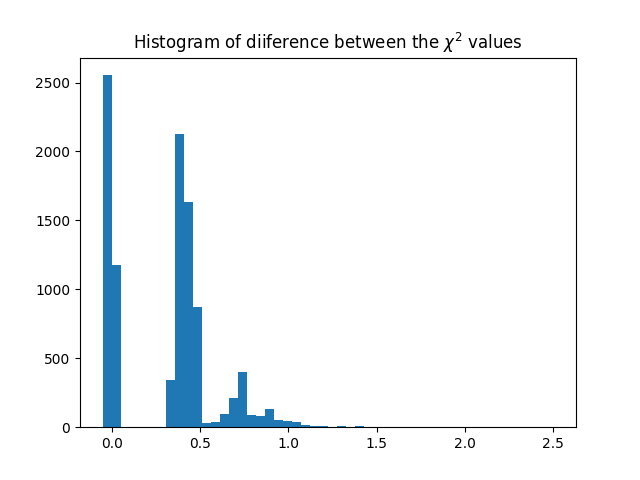
\includegraphics[scale =0.7]{csq_hist_edges.png}
\caption[Histogram of Chi-Square of drawn samples]{Histogram of Chi-Square of drawn samples, the mean is 49.20 with standard deviation of 41.98.}
\label{fig:csq_hist_known_curve}
\end{figure}

\begin{figure}[h!]
\centering
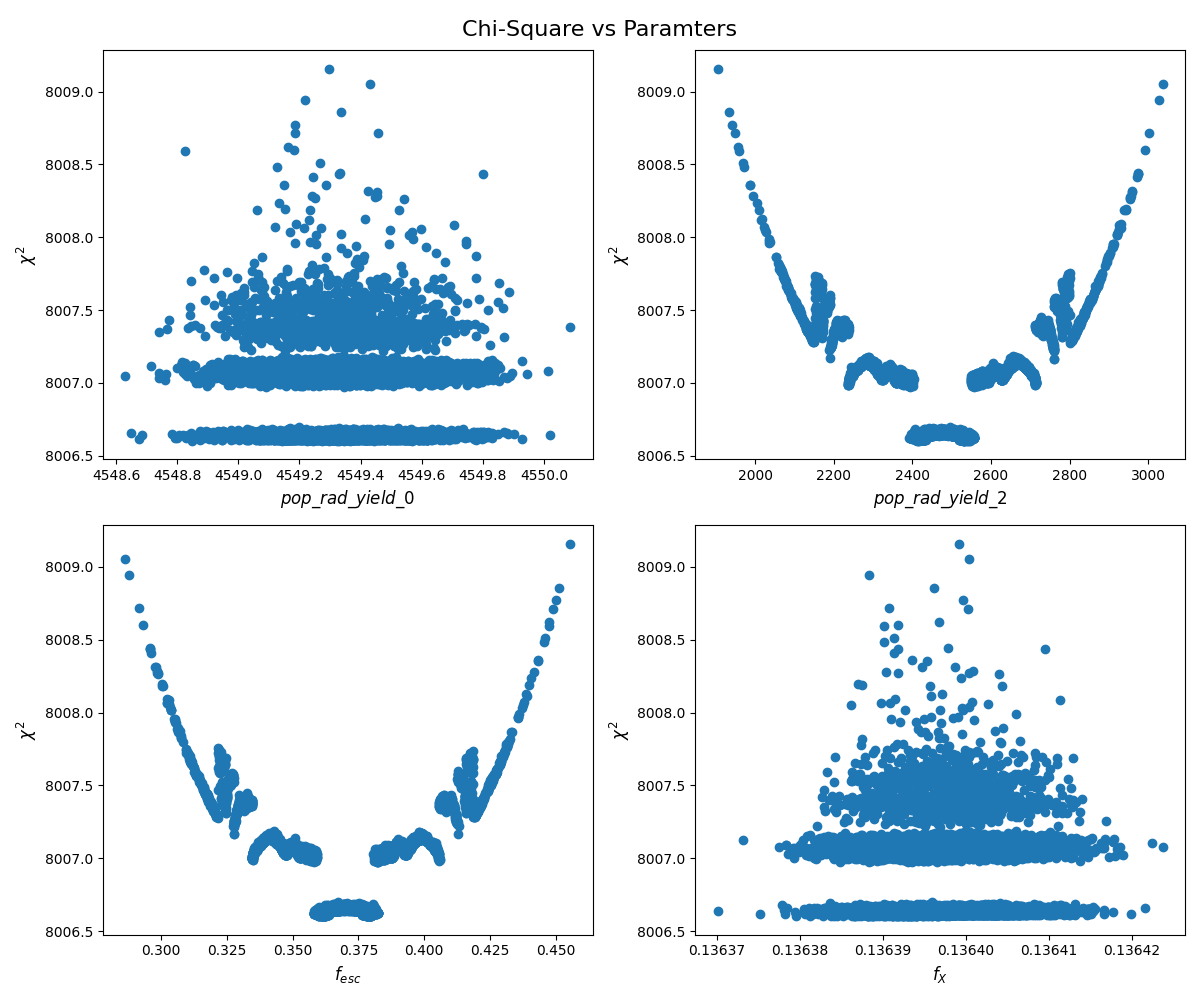
\includegraphics[scale =0.5]{csq_vs_params_edges.png}
\caption[Chi-Square of Drawn samples vs parameter values]{Chi-Square of Drawn samples versus parameter values for a known ARES curve with four parameters, The parabolic behaviour is not obvious in these plots.}
\label{fig:csq_vs_params_knwon_curve}
\end{figure}

\begin{figure}[h!]
\centering
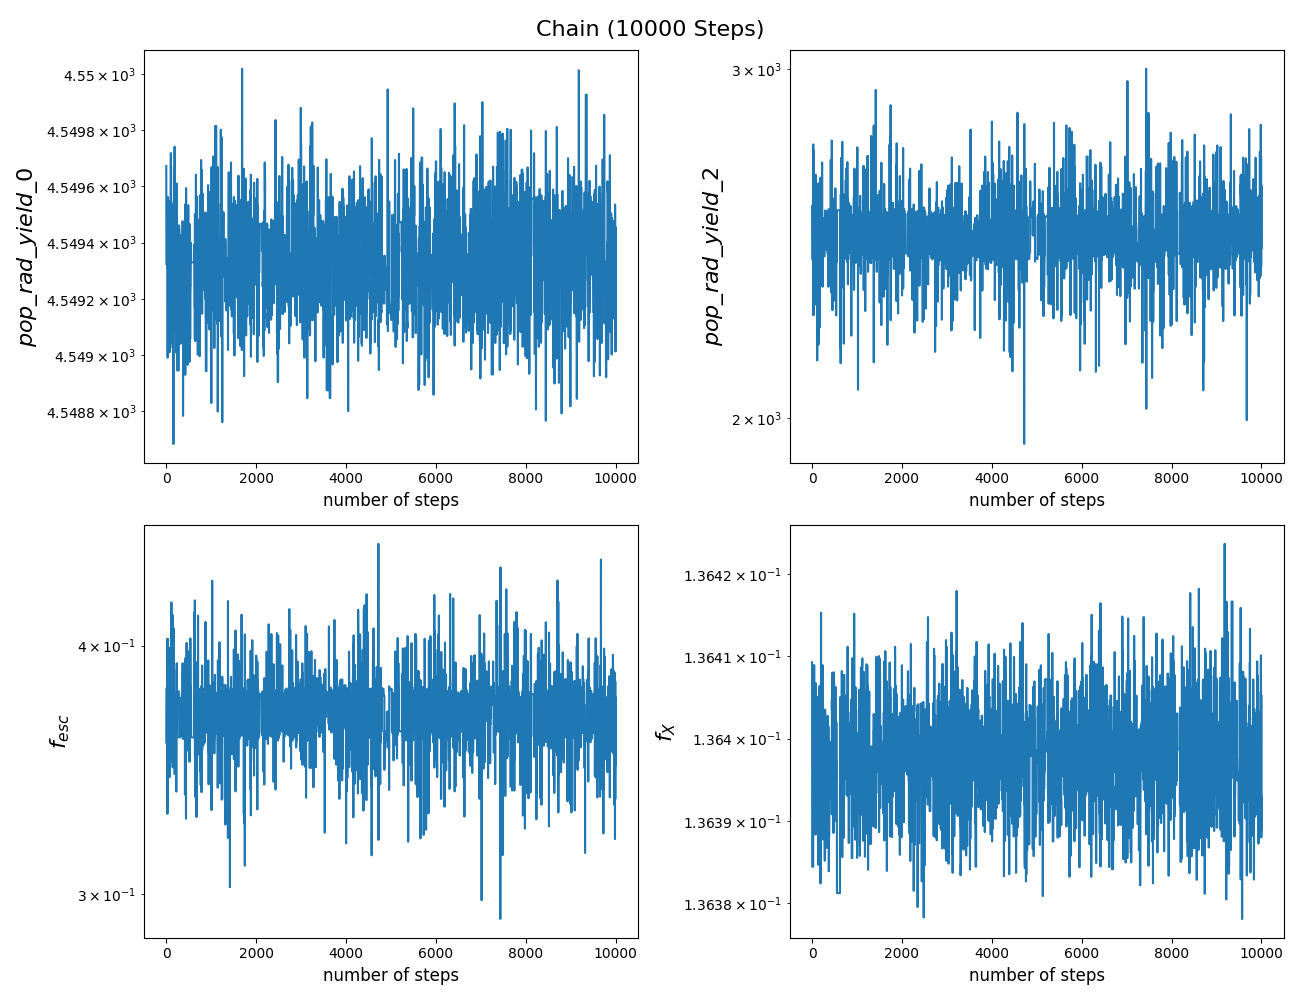
\includegraphics[scale =0.5]{chain_edges.png}
\caption[Trend of parameters]{Trend of parameters in the MCMC chain, White noise behaviour is considered as a sign of convergence. The acceptance ratio of the chain is $22.12\%.$}
\label{fig:chain_known_curve}
\end{figure}

\begin{figure}[h!]
\centering
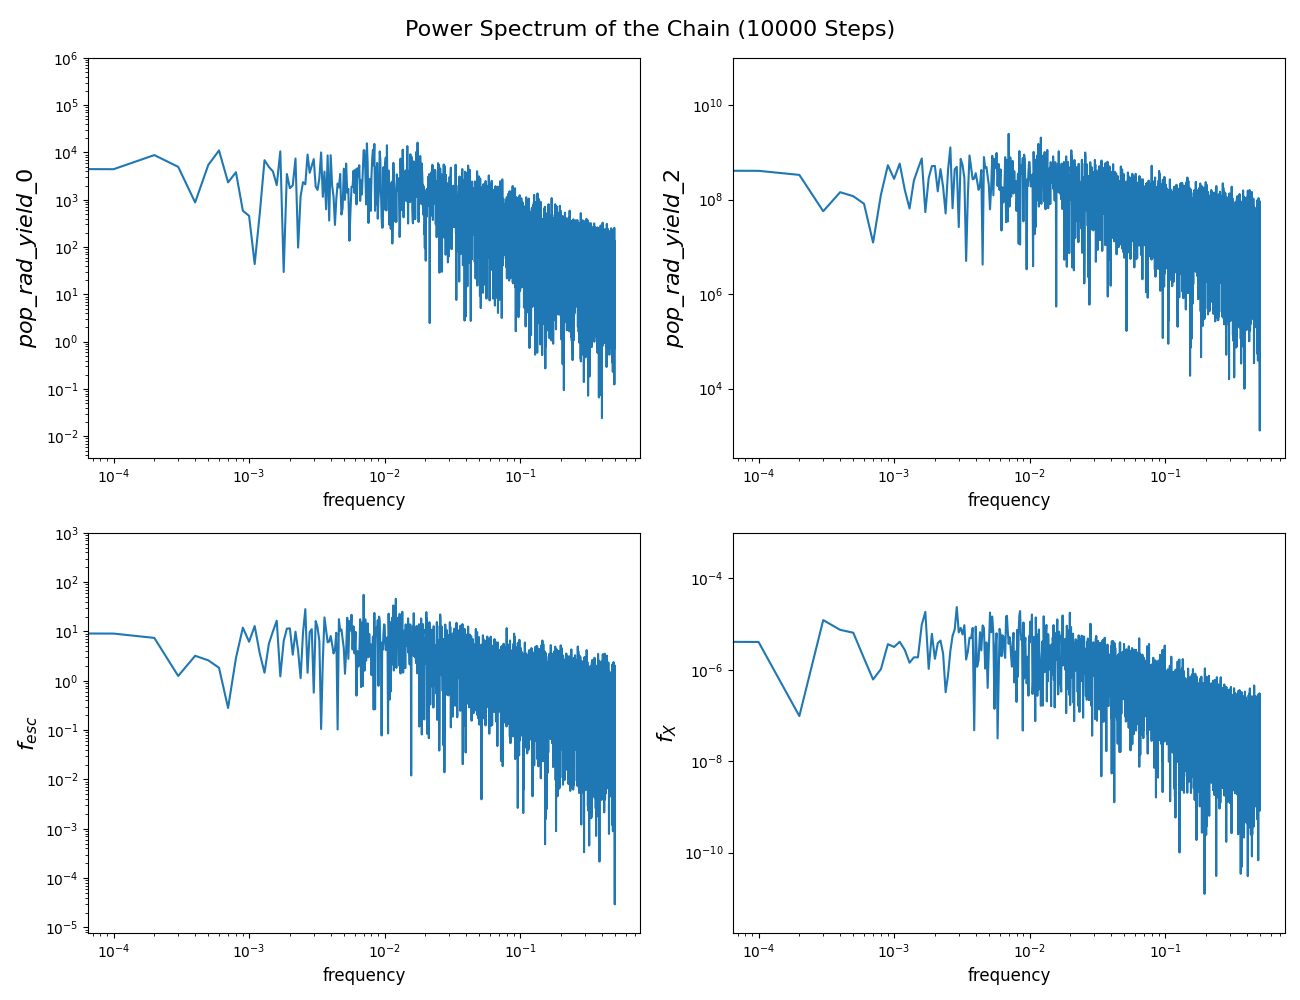
\includegraphics[scale =0.5]{power_spectrum_edges.png}
\caption[Power spectrum of the chain]{Power spectrum of the chain, Flat behaviour in low frequencies is in agreement with results of \ref{fig:chain_known_curve}.}
\label{fig:power_spectrum_known_curve}
\end{figure}

\begin{figure}[h!]
\centering
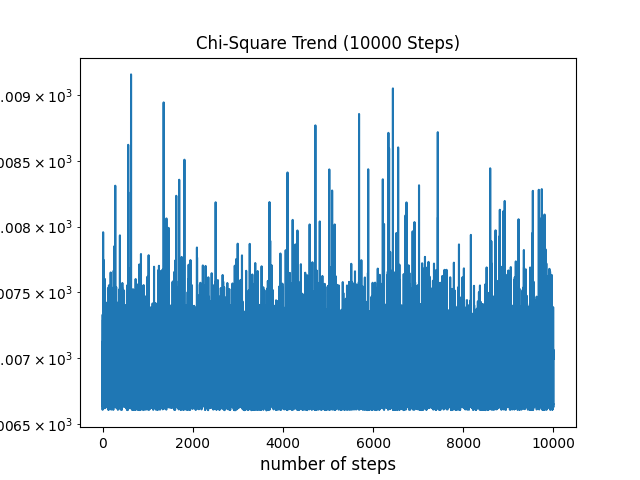
\includegraphics[scale =0.6]{csq_trend_edges.png}
\caption[Trend of chi-square]{Trend of chi-square in the MCMC chain, The chain seems to have reached an equilibrium state.}
\label{fig:csq_trend_knwon_curve}
\end{figure}

\begin{figure}[h!]
\centering
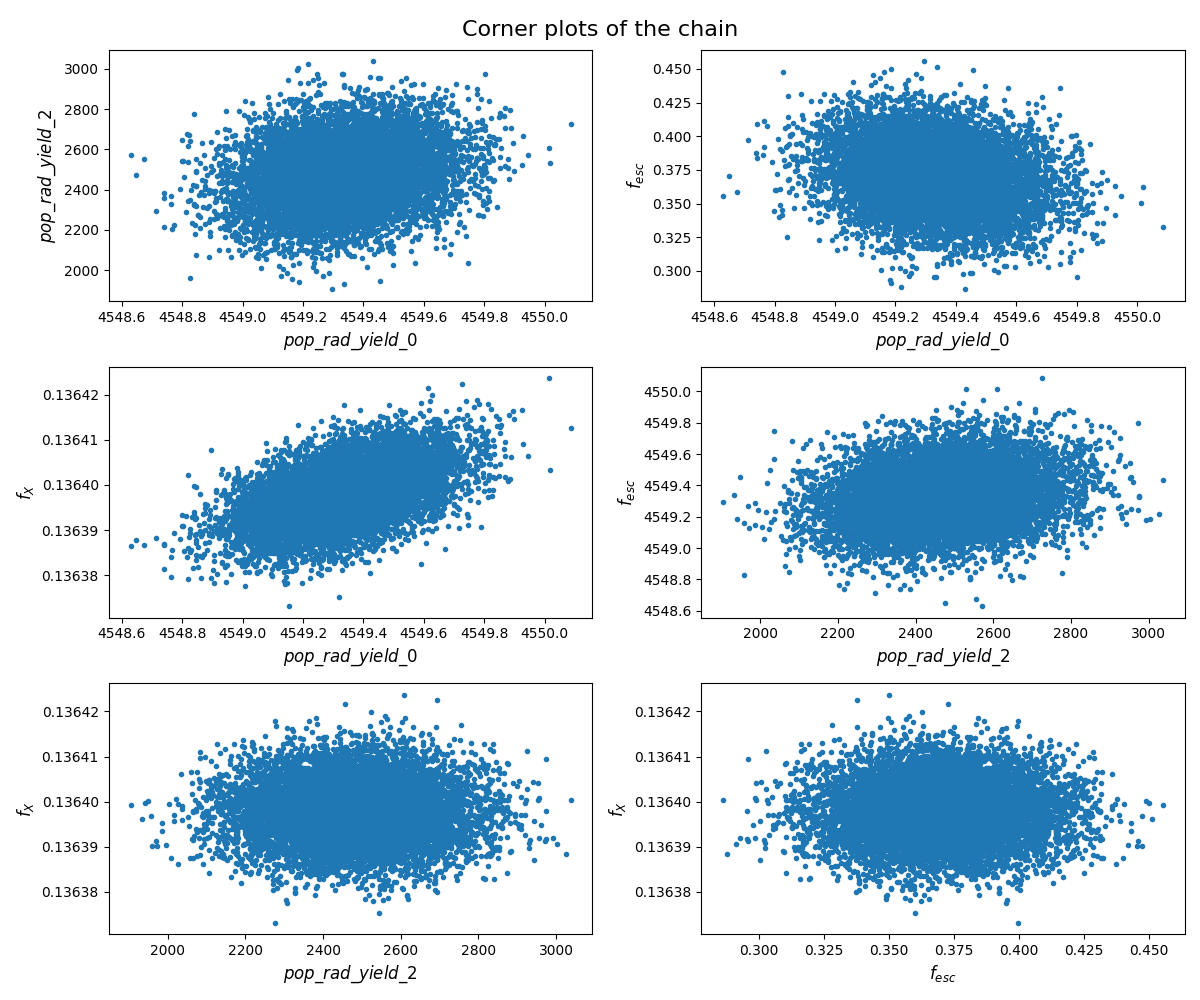
\includegraphics[scale =0.5]{corner_plots_edges.png}
\caption[Corner plots of the chain]{Corner plots of the chain indicating the correlation between the parameters specially in the lower left panel}
\label{fig:corner_plots_known_curve}
\end{figure}
%###################################################################################
\chapter{Discussion and Conclusion}
\label{chap:discussion}
\section{Interpretation of the results}
%\section{Implications for cosmology and astrophysics}
\section{Summary of the main findings}
\section{Comparison with previous studies and observations}
\section{Contributions and significance of the research}
\section{Limitations}
We faced certain limitation while working on this research. Most of those emerged during the implementation of python script. 
An strongly limiting obstacle is related to the ARES's run time which is in the order of a few seconds per each simulation (approximately 4 to 5 seconds for different combination of parameters). Given that ARES is computationally heavy, it will make it hard to use algorithms based on using ARES on each iteration \footnote{ As an example, the run time for the MCMC results presented in chapter \ref{chap:results} was approximately 13 hours.}. This was main the reason that led us to combine the MCMC with LM in order to have a more efficient chain and guarantee the convergence.\par 
%----------------------------------------------------------------------------
\section{Future work}
As the first step, the developed script is going to be published as a python package in near future. There will be a corresponding paper describing a summary of the results shown in chapter \ref{chap:results}.\par
We plan to take the analysis further and include a realistic foreground model. Then, we will add some of the previously mentioned non-standard effects to ARES simulations and run the same described method to observe the difference the best-fit curve. \hl{The results will hopefully tell us if existing and future observational data (like EDGES) is a sign of new physics and can be explained through physics beyond standard cosmological model.}\par

%##############################################################################
\chapter{Appendices}
\section{Derivation of radiometer equation}
\section{Code snippets and scripts}	
\subsection{Levenberg-Marquardt}
\label{chap:appendix,sub:LM}
\subsection{Markov Chain Monte Carlo}
\label{chap:appendix,sub:MCMC}
\subsection{drawing samples from covariance matrix}
\label{chap:appendix,sub:draw}

	% Begin Bibliography
	{
	
	\bibliography{references}
	\bibliographystyle{ieeetr}
	
	}
\end{document}